% !TEX encoding = UTF-8 Unicode
\chapter{Simulation results}  \label{chap-simulation}

This chapter describes numerical simulations carried out to demonstrate and evaluate the disturbance models and observer designs described in Chapter \ref{chap-methods}. Section \ref{section:sim-RODDs} describes simulated examples of different RODDs. Section \ref{section:sim-obs-lin} describes experiments to evaluate the two observers in estimating the states of two simulated systems, a single-input single-output (SISO) linear system with one RODD step disturbance, followed by a 2-input, 2-output linear system with two RODD step disturbances. Section \ref{section:sim-ore-SISO} describes an experiment to evaluate the observers on the simulated grinding circuit model with one output variable and a step disturbance in the ore feed mix. Section \ref{section:sim-ore-mimo-ctrl} describes an experiment to evaluate the observers in a multi-variable feedback control scenario with the simulated grinding circuit model.


\section{Generating RODD disturbances} \label{section:sim-RODDs}

RODDs are easy to generate by numerical simulation.  Plot (a) in Figure \ref{fig:rodd-sim-plots} shows a random shock sequence (\ref{eq:wpk1}) of length 1000 samples generated using a pseudo random number generator. Plots (b), (c), and (d) show step, ramp and exponential change disturbances generated with this random shock sequence using the RODD models in (\ref{eq:RODD-step}), (\ref{eq:RODD-ramp}), and (\ref{eq:RODD-exp}). 
\begin{figure}[htp]
	\centering
	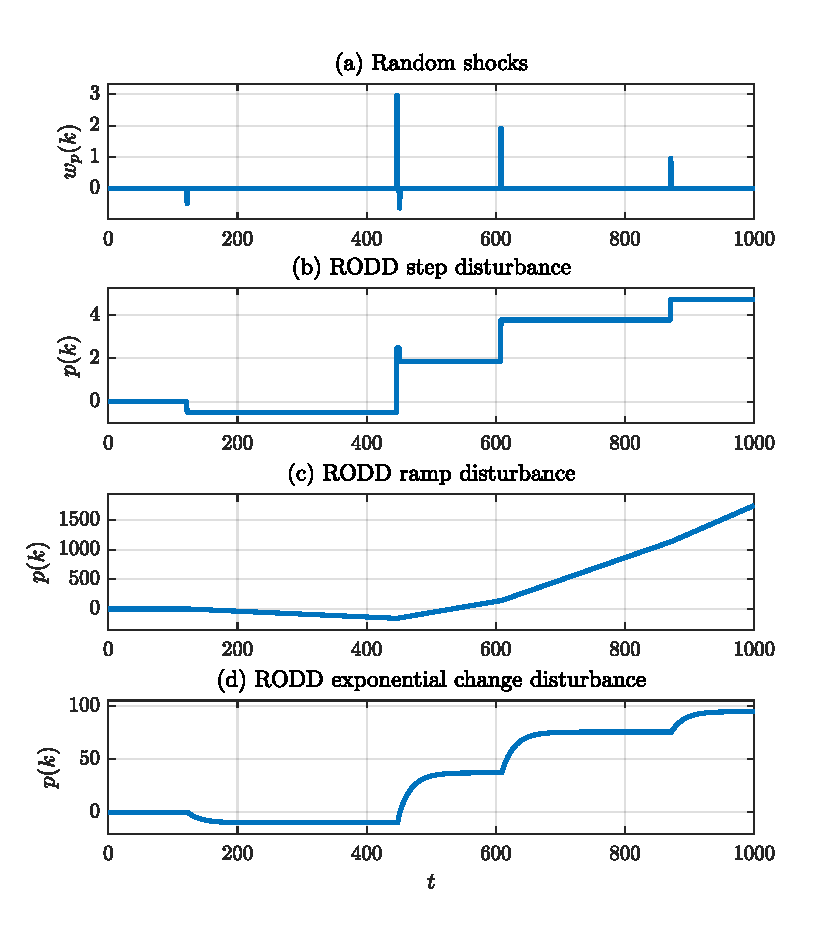
\includegraphics[width=13cm]{images/rodd_sim_plots.pdf}
	\caption{Examples of RODDs}
	\label{fig:rodd-sim-plots}
\end{figure}
\begin{figure}[htp]
	\centering
	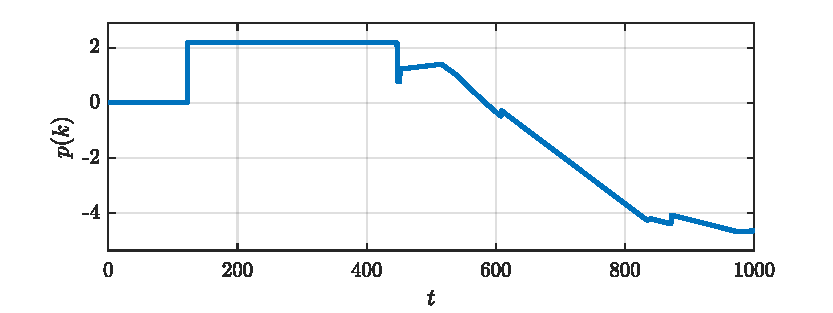
\includegraphics[width=13cm]{images/rodd_sim_plot2.pdf}
	\caption{A RODD with steps and ramps}
	\label{fig:rodd-sim-plot2}
\end{figure}


\section{Observer evaluation with linear systems} \label{section:sim-obs-lin}

\subsection{SISO linear system} \label{sim-obs-lin-1}

To demonstrate state estimation in the presence of RODDs, a single RODD was simulated at the input to a SISO process represented by a discrete-time linear model, as shown in the functional diagram in Figure \ref{fig:sim-sys-diag-siso}. In addition to the unmeasured RODD, $p(k)$, the process has a known input variable, $u(k)$, and a measured output variable, $y_M(k)$. The measurements are simulated by adding a random noise $v(k)$ with zero mean and standard deviation $\sigma_M$ to the output of the process. At each sample time, the input and measured output are passed to an observer which calculates estimates of the process states, $\hat{\mathbf{x}}(k|k)$, and an estimate of the true process output, $\hat{y}(k|k)$, at the current time.
\begin{figure}[htp]
	\centering
	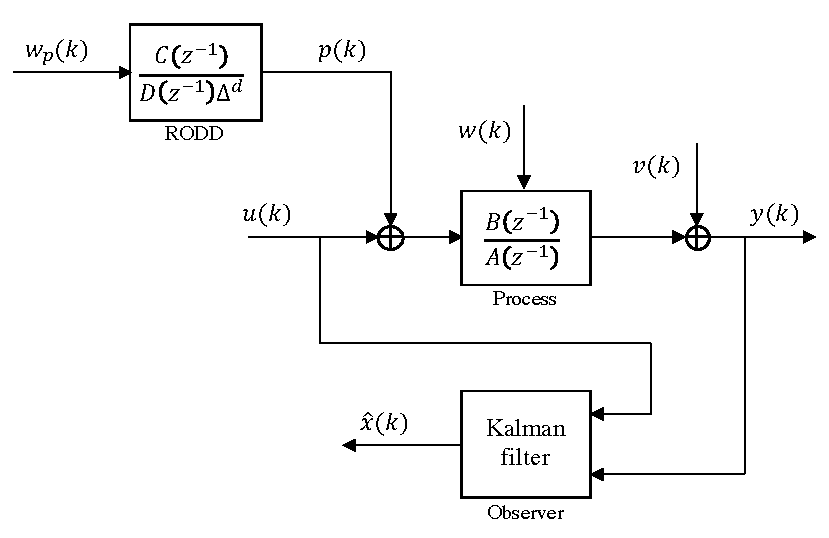
\includegraphics[width=11.5cm]{images/sim-sys-diag-siso.pdf}
	\caption{Functional diagram of the simulated SISO system with observer}
	\label{fig:sim-sys-diag-siso}
\end{figure}

For the purposes of this experiment, the linear model used to represent the process was the stable first order system,
\begin{equation}
	\frac{B(z^{-1})}{A(z^{-1})} = \frac{0.3z^{-1}}{1-0.7z^{-1}}
\end{equation}
with a sampling period of $T=0.5$.

The RODD was a step disturbance created by setting
\begin{equation}
	\frac{C(z^{-1})}{D(z^{-1})} = \frac{1}{1-z^{-1}}.
\end{equation}
The random shock, $w_p(k)$, was defined by (\ref{eq:wpik2}) with $\epsilon=0.01$, $\sigma_{w_p}=0.01$, and $b=100$.

The state-space representation used to simulate the augmented system was
\begin{equation} \label{eq:sim-sys-siso-ss-aug}
	\begin{split}
	\mathbf{x}_{a}(k+1) & =\left[\begin{array}{cc}
		0.7 & 1 \\
		0 & 1
	\end{array}\right] \mathbf{x}_{a}(k)+\left[\begin{array}{l}
		1 \\
		0
	\end{array}\right] u(k) + \mathbf{w}_{a}(k) \\
	y(k) & =\left[\begin{array}{cc}
	0.3 & 0
\end{array}\right] \mathbf{x}_{a}(k) + v(k)
\end{split}
\end{equation}
where
\begin{equation} \label{eq:sim-sys-siso-ss-aug2}
		\mathbf{x}_{a}(k) = \left[\begin{array}{l}
			x_{a,1}(k) \\
			x_{a,2}(k)
		\end{array}\right] = \left[\begin{array}{l}
		x_{1}(k) \\
		p(k)
	\end{array}\right], \mathbf{w}_{a}(k) = \left[\begin{array}{l}
	w_1(k) \\
	w_{p}(k)
\end{array}\right] .
\end{equation}

Note that with this representation, the second model state $x_{a,2}(k)$ corresponds exactly to the input disturbance $p(k)$.

\subsection{Analysis of sub-optimal estimators} \label{sim-obs-lin-1-SKF-analysis}

\begin{figure}[htp]
	\centering
	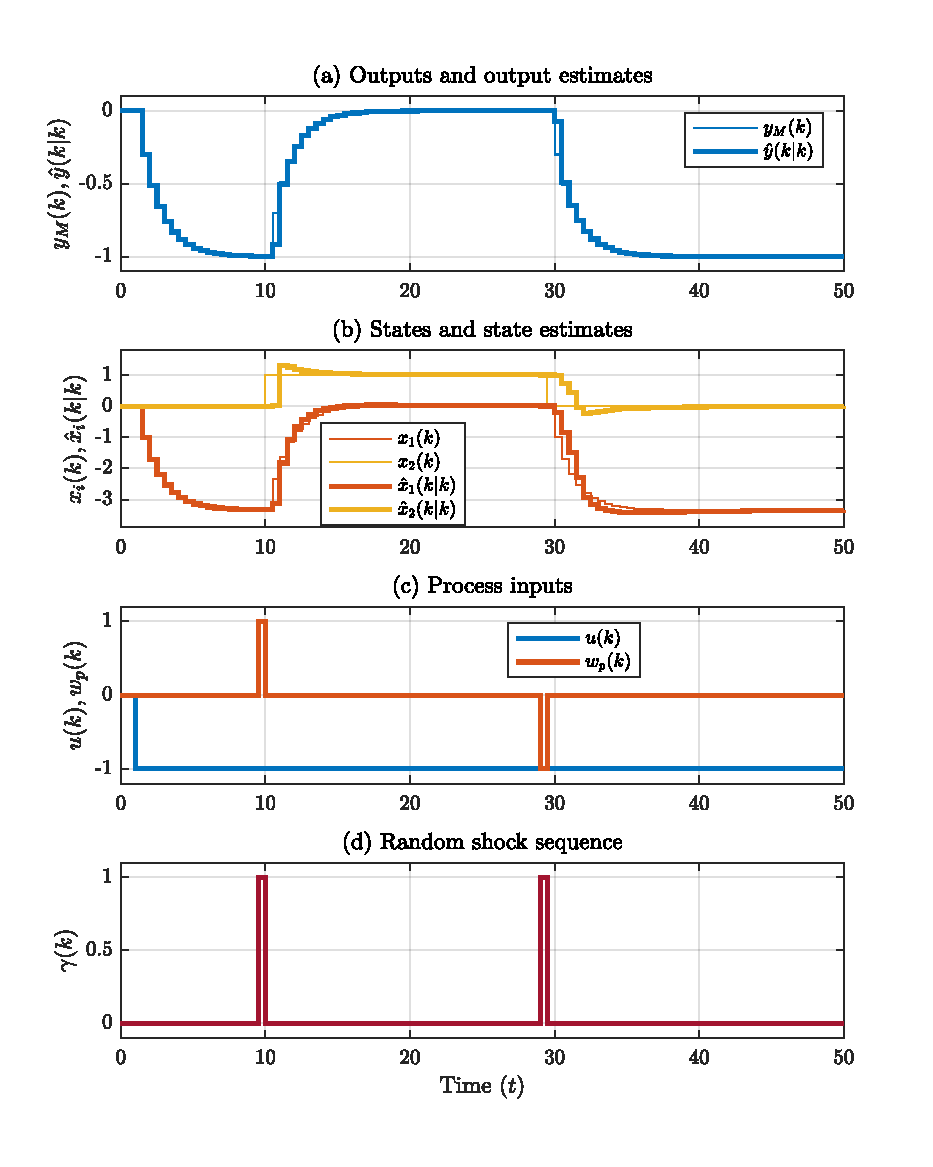
\includegraphics[width=13cm]{images/rod_MKF_SF_test_sim_MKF_SF95_ioplot.pdf}
	\caption{Simulation of a SISO linear system with a RODD input disturbance}
	\label{fig:rod-obs-sim-test-ioplot-SF95}
\end{figure}
To investigate the behaviour and internal workings of the observers, the system (\ref{eq:sim-sys-siso-ss-aug}) was simulated with one pre-determined shock, no persistent disturbance ($\sigma_{w_p}=0$), and no measurement noise. Figure \ref{fig:rod-obs-sim-test-ioplot-SF95} shows the inputs and outputs of this simulation, which was 100 sample periods in duration. The two lower subplots show the system inputs, including the random shock signal. The upper two plots show the system states and outputs as well as the estimates of the states and outputs by the multi-model observer using sequence fusion \citep{robertson_detection_1995}.

\begin{figure}[htp]
	\centering
	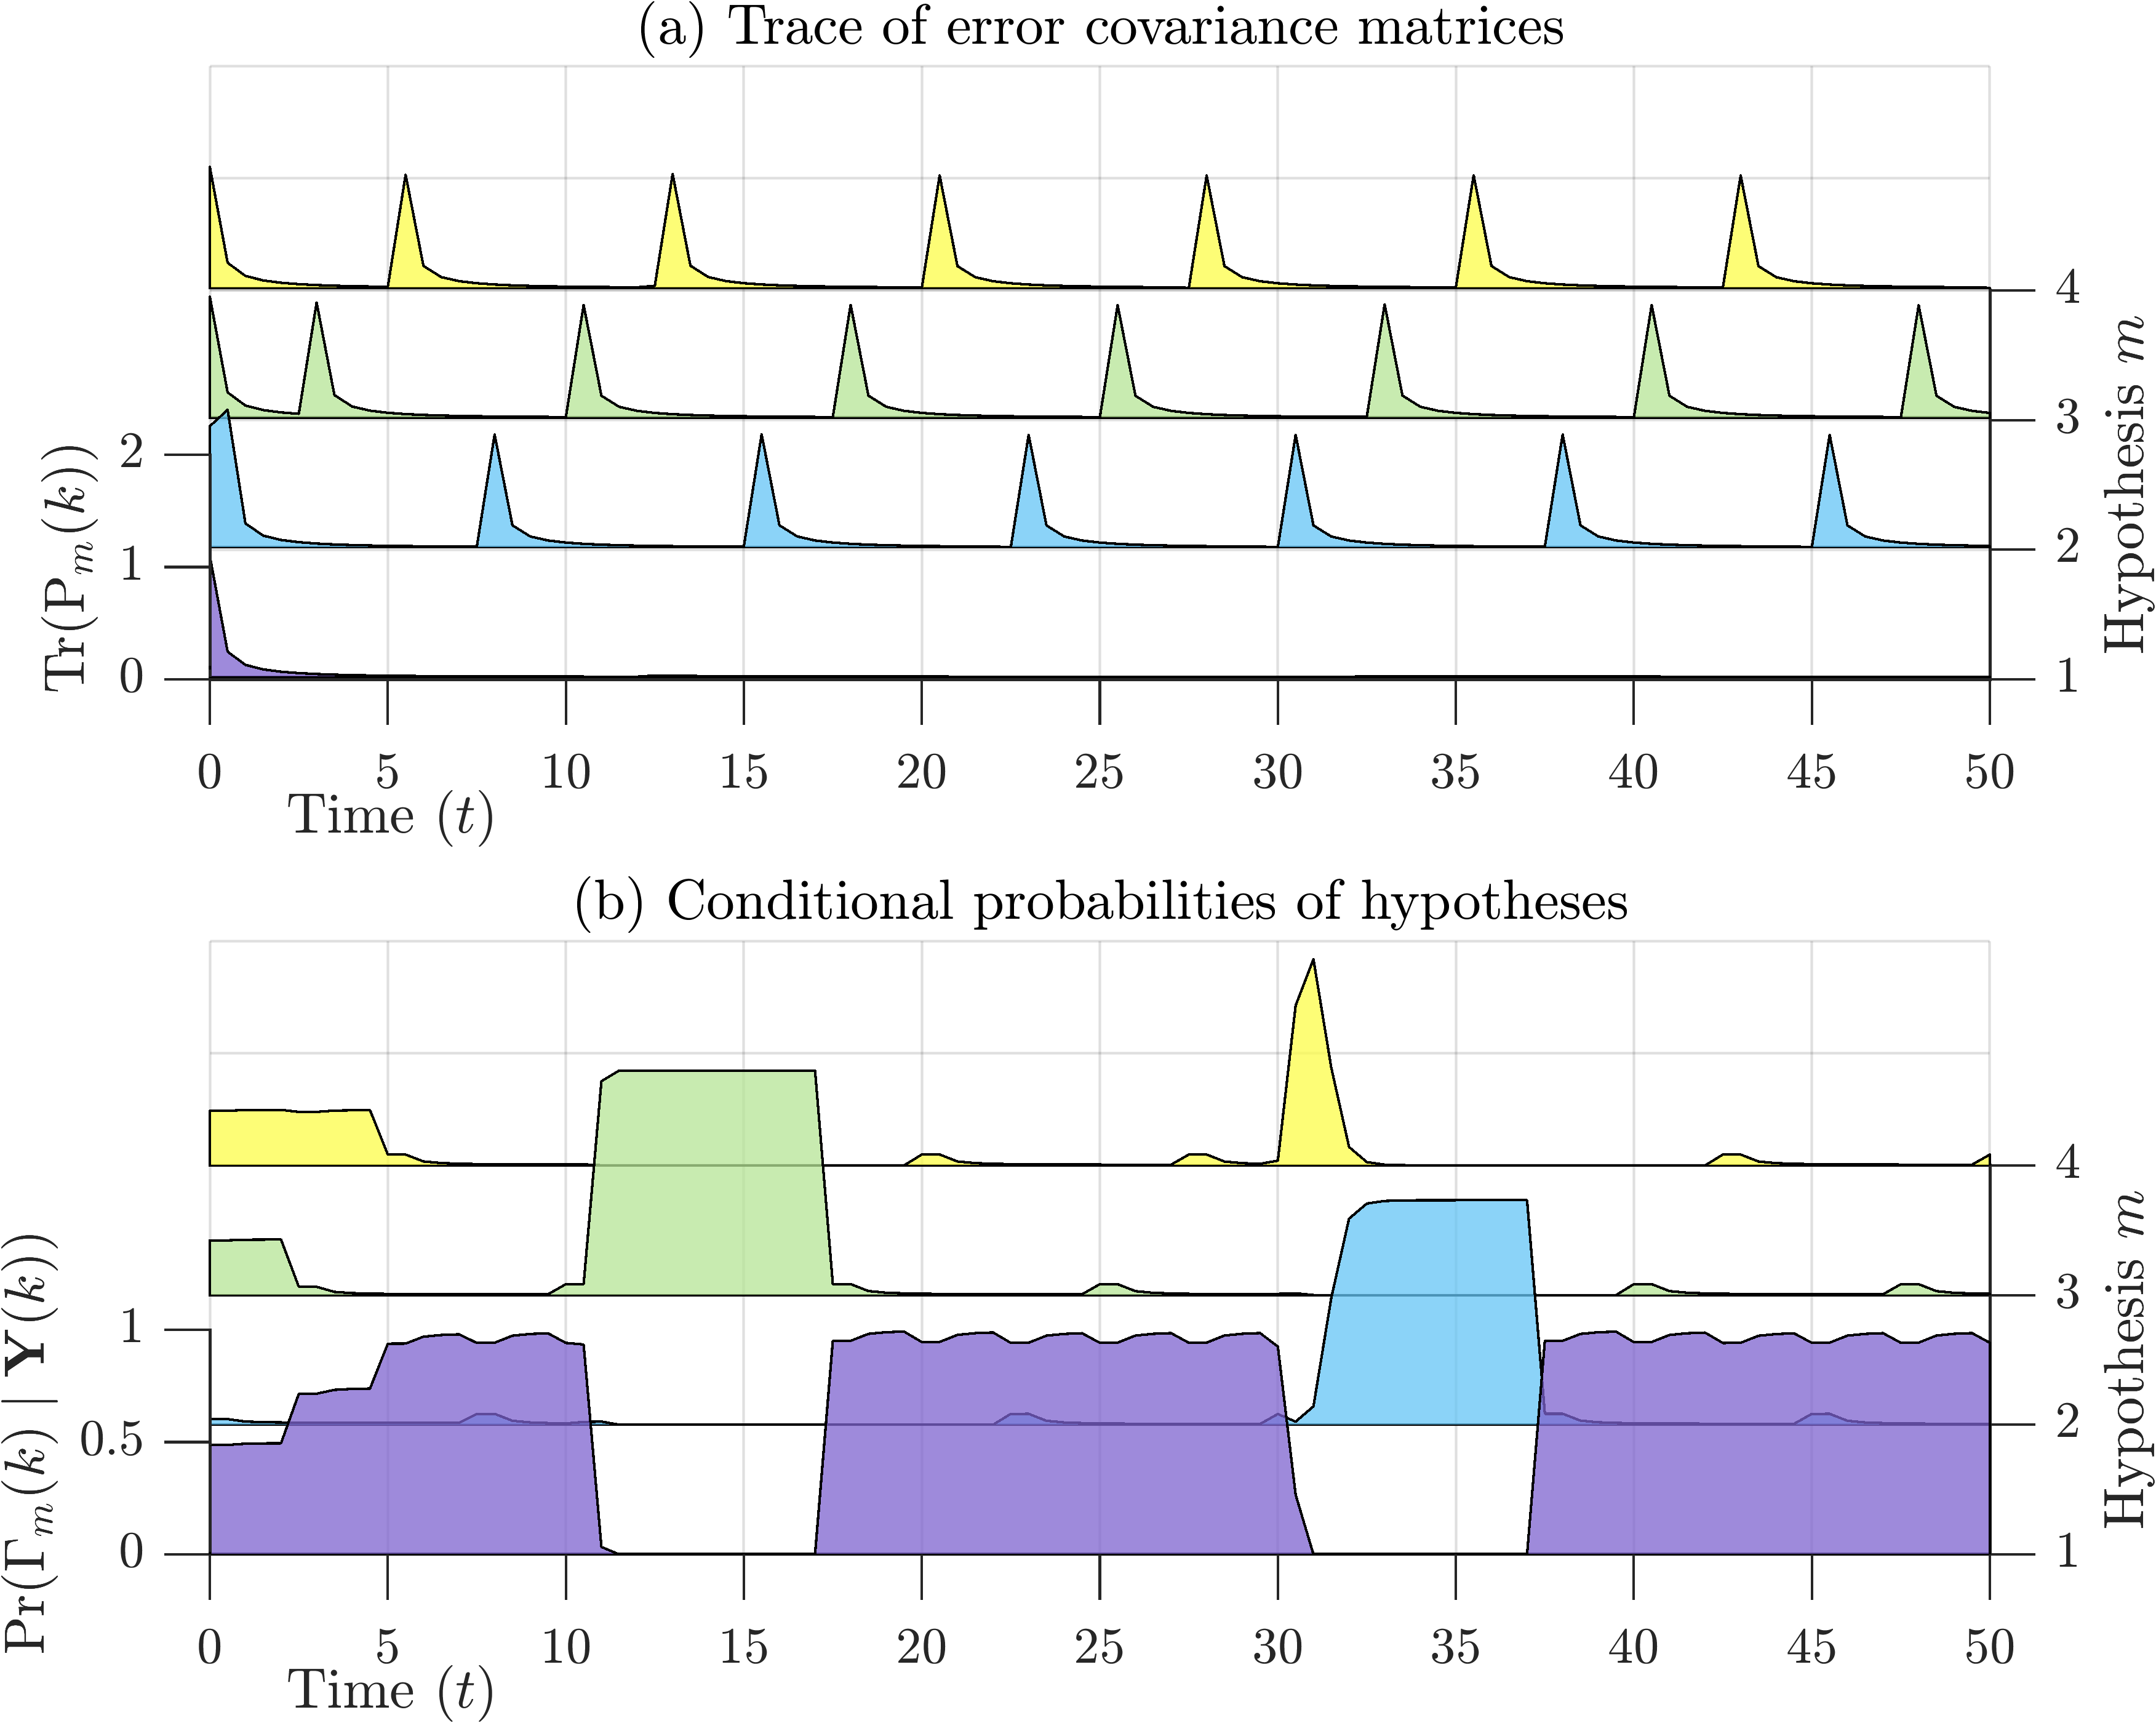
\includegraphics[width=12cm]{images/rod_MKF_test_sim_MKF_SF95_prob.png}
	\caption{Multi-model observer probability estimates – MKF-SF95}
	\label{fig:rod-obs-sim-test-probs-SF95}
\end{figure}
The two subplots in Figure \ref{fig:rod-obs-sim-test-probs-SF95} provide insight into the computations of this observer which is labelled `MKF-SF95'. The upper plot shows four time series of the trace (i.e. the sum of the elements on the main diagonal) of the error covariance matrices, $\mathbf{P}_f(k)$, of the state estimates of each filter. The diagonal values of $\mathbf{P}_f(k)$ may be interpreted as indications of the magnitude of the expected errors in the state estimates. Recall that $\mathbf{P}_f(k+1)$ is only a function of the value at the current time, $\mathbf{P}_f(k)$, and the switching process noise covariance, $\mathcal{Q}(\gamma_f(k))$ (\ref{eq:Pfk}). The lower plot shows the likelihood estimates of the hypothesis sequences conditioned on the data up to time $k$ (\ref{eq:Pr_Gammak_given_Yk}).

In this simulation, the error covariances at time $t=0$ were initialized to the identify matrix and the conditional likelihoods were initialized to equal values (i.e. $\mathbf{P}_f(0)=\mathbf{I}_2,\operatorname{Pr}\left(\Gamma_f(0) \mid \mathbf{Y}(0)\right)=0.25$, for $f=1,2,...,n_h$). In the upper plot it can be seen that the $\operatorname{Tr}(\mathbf{P}_f(k))$ initially drop rapidly and tend towards zero, however, at certain times, they increase sharply to a peak before dropping again. The sharp peaks are caused by the assumption of shocks ($\gamma_f(k)=1$) at pre-determined times in the hypothesis sequences of each filter. However, the error covariance of filter 1 drops to zero and never increases because this filter represents the hypothesis that no shocks occur at any time.

From the lower plot, it can be seen that the likelihoods of each filter fluctuate initially then settle on a steady-state by $t=5$. Between $t=5$ and $t=10$, filter 1 has a likelihood close to 1 and the others are close to zero, which means that the estimates of the observer are determined almost completely by filter 1. This makes sense since no shocks have occurred at this point in time. The simulated shock actually occurs at $t=9.5$. Hypothesis sequence 3 assumes a shock at $t=10$ ($\gamma_3(10)=1$) and thus the error covariance increases at $t=10.5$ and peaks at $t=11$. From the lower plot, it can be seen that the likelihood switches from filter 1 to filter 3 at $t=12$ and the likelihood of filter 3 is 1 for the remainder of the simulation.

\begin{figure}[htp]
	\centering
	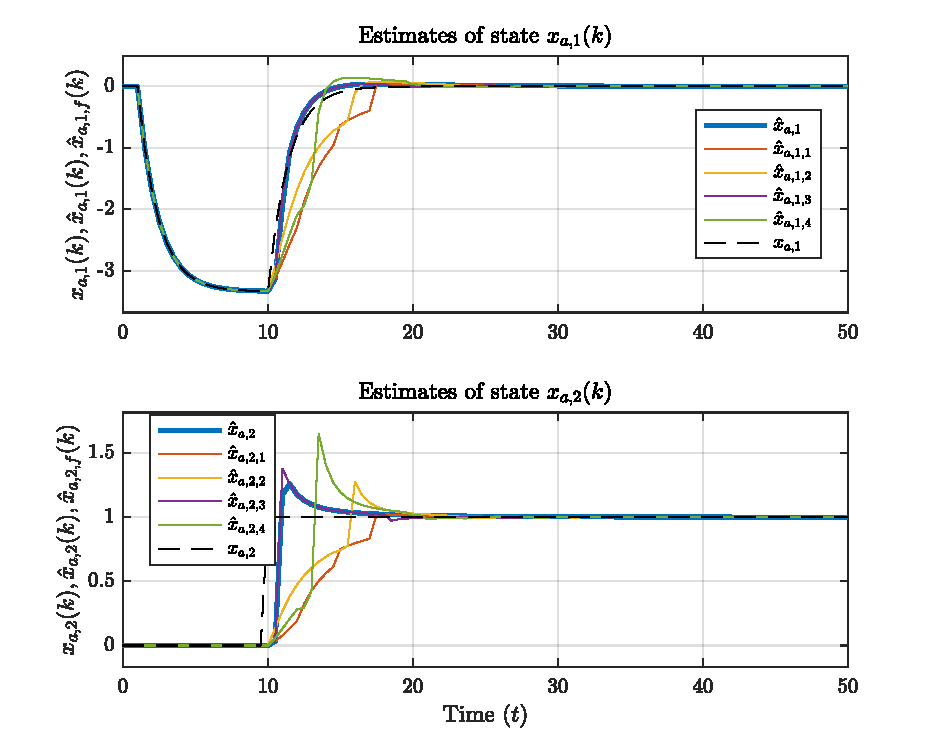
\includegraphics[width=13cm]{images/rod_MKF_test_sim_MKF_SF95_x_est.pdf}
	\caption{Multi-model observer state estimates – MKF-SF95}
	\label{fig:rod-obs-sim-test-x_est-SF95}
\end{figure}
Figure \ref{fig:rod-obs-sim-test-x_est-SF95} shows the state estimates of all 4 filters, as well as the overall state estimates calculated from the hypothesis likelihoods, and the true values of the system states. These plots reveal the role that each filter estimate plays in the overall estimates. The estimates of the filter 3 (purple lines) are the first to respond to the shock occurrence. The other estimates (green, yellow and orange lines) respond at later intervals and filter 1 (orange lines) takes the longest to respond. After filter 3 has corrected its estimates in response to the change in the output, the overall estimates (thick blue lines) switch from filter 1 to filter 3 in one time-step.

As described in Section \ref{subsec-fusion}, Robertson and coworkers proposed an alternative implementation of the sequence fusion algorithm in their 1998 paper. There are two differences between this and the previous algorithm. Firstly, shocks are assumed to act over the duration of the detection interval rather than at one sample time within the interval. Secondly, the probability and variance of the shock signal, $w_{p}(k)$, are adjusted (\ref{eq:deltak}, \ref{eq:wpdk}).

\begin{figure}[htp]
	\centering
	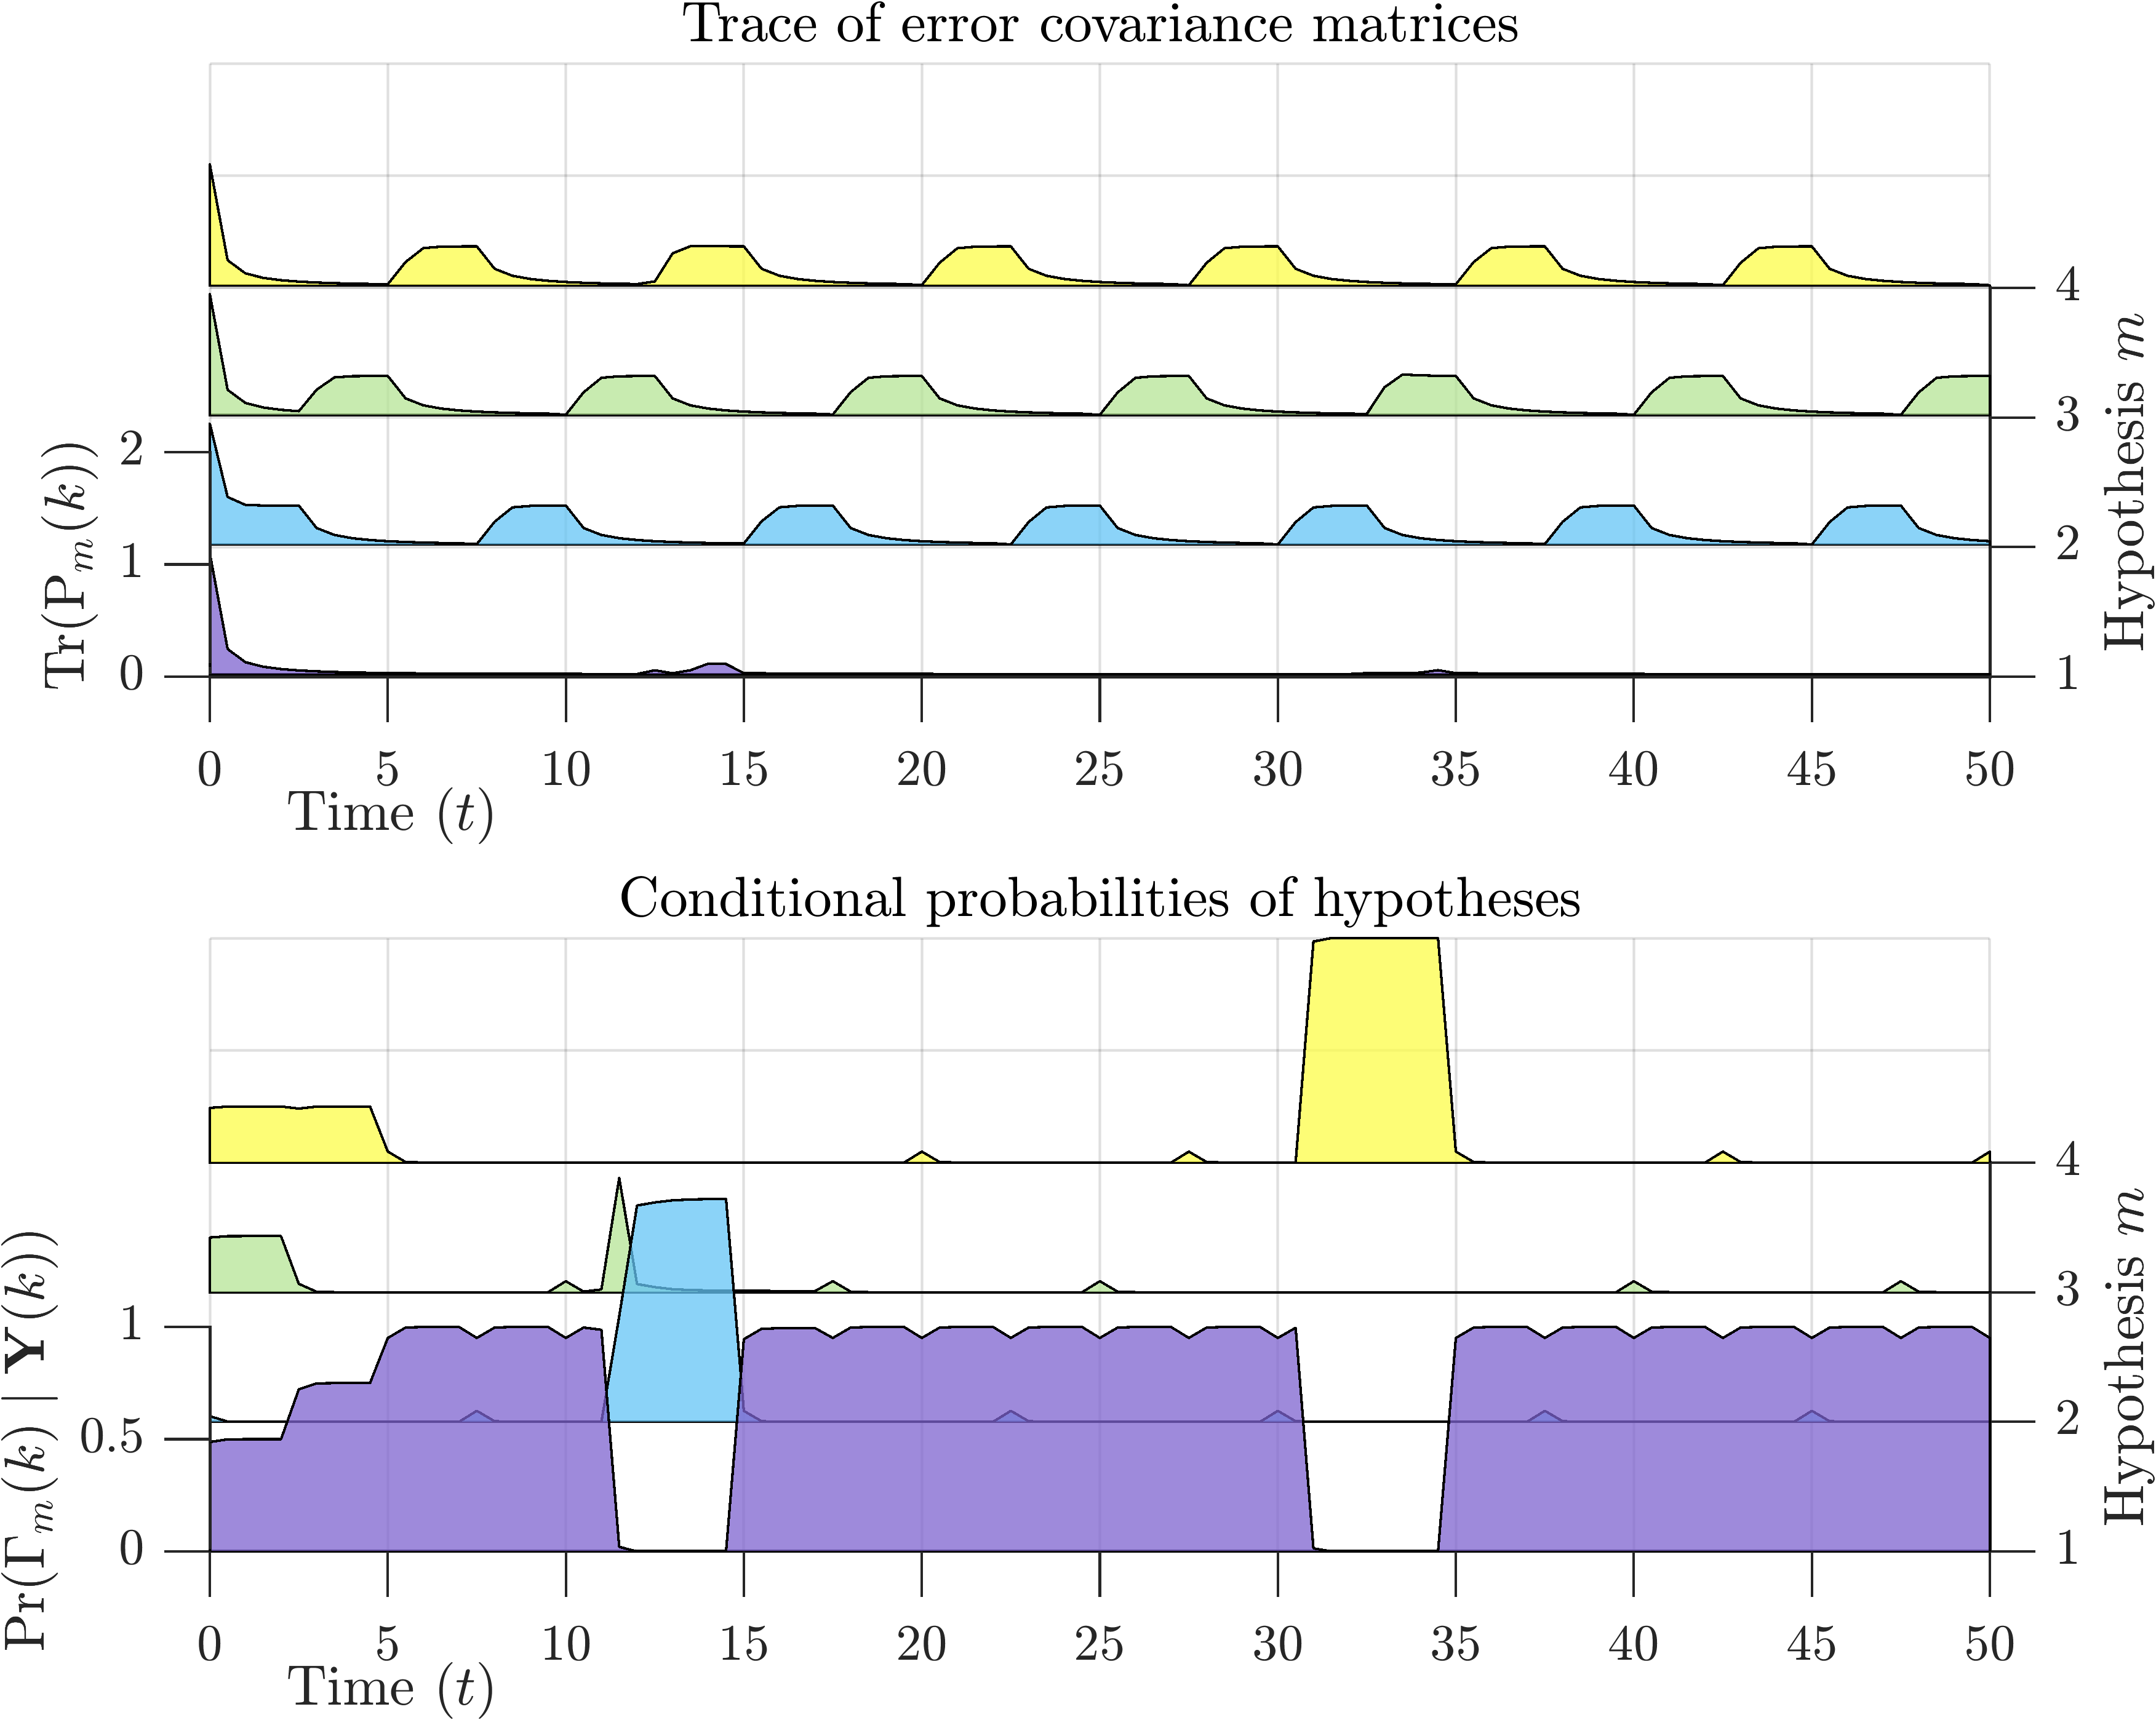
\includegraphics[width=12cm]{images/rod_MKF_test_sim_MKF_SF98_prob.png}
	\caption{Multi-model observer probability estimates – MKF-SF98}
	\label{fig:rod-obs-sim-test-probs-SF98}
\end{figure}
Figures \ref{fig:rod-obs-sim-test-probs-SF98} and \ref{fig:rod-obs-sim-test-x_est-SF98} show the results of simulating the 1998 version of the observer (labelled `MKF-SF98') with the same simulation data. The effect of the modification on the covariance matrices is very clear. The traces peak at a lower value and the peak is sustained for a number of sample periods before declining. The effect of this modification on the observer estimates is less clear. The hypothesis likelihood switches from filter 1 to filter 2 at around $t=13$, then alternates between filters 2 and 3 for the remainder of the simulation. In the case of this simulation, the response to the shock is slower and the errors in the output estimates are higher.
\begin{figure}[htp]
	\centering
	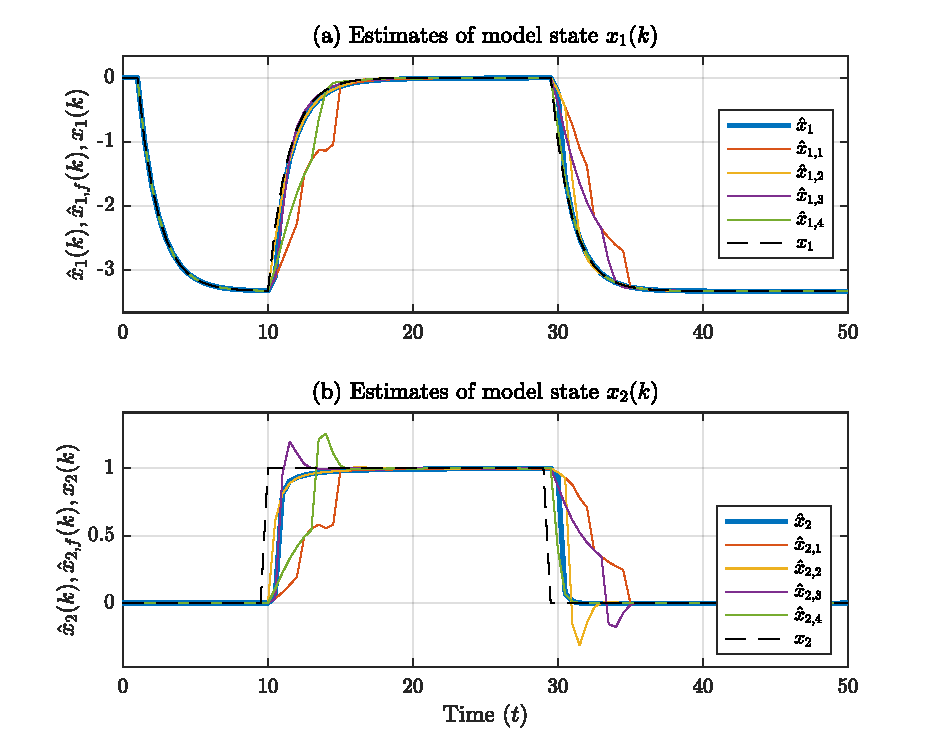
\includegraphics[width=13cm]{images/rod_MKF_test_sim_MKF_SF98_x_est.pdf}
	\caption{Multi-model observer state estimates – MKF-SF98}
	\label{fig:rod-obs-sim-test-x_est-SF98}
\end{figure}

\begin{figure}[htp]
	\centering
	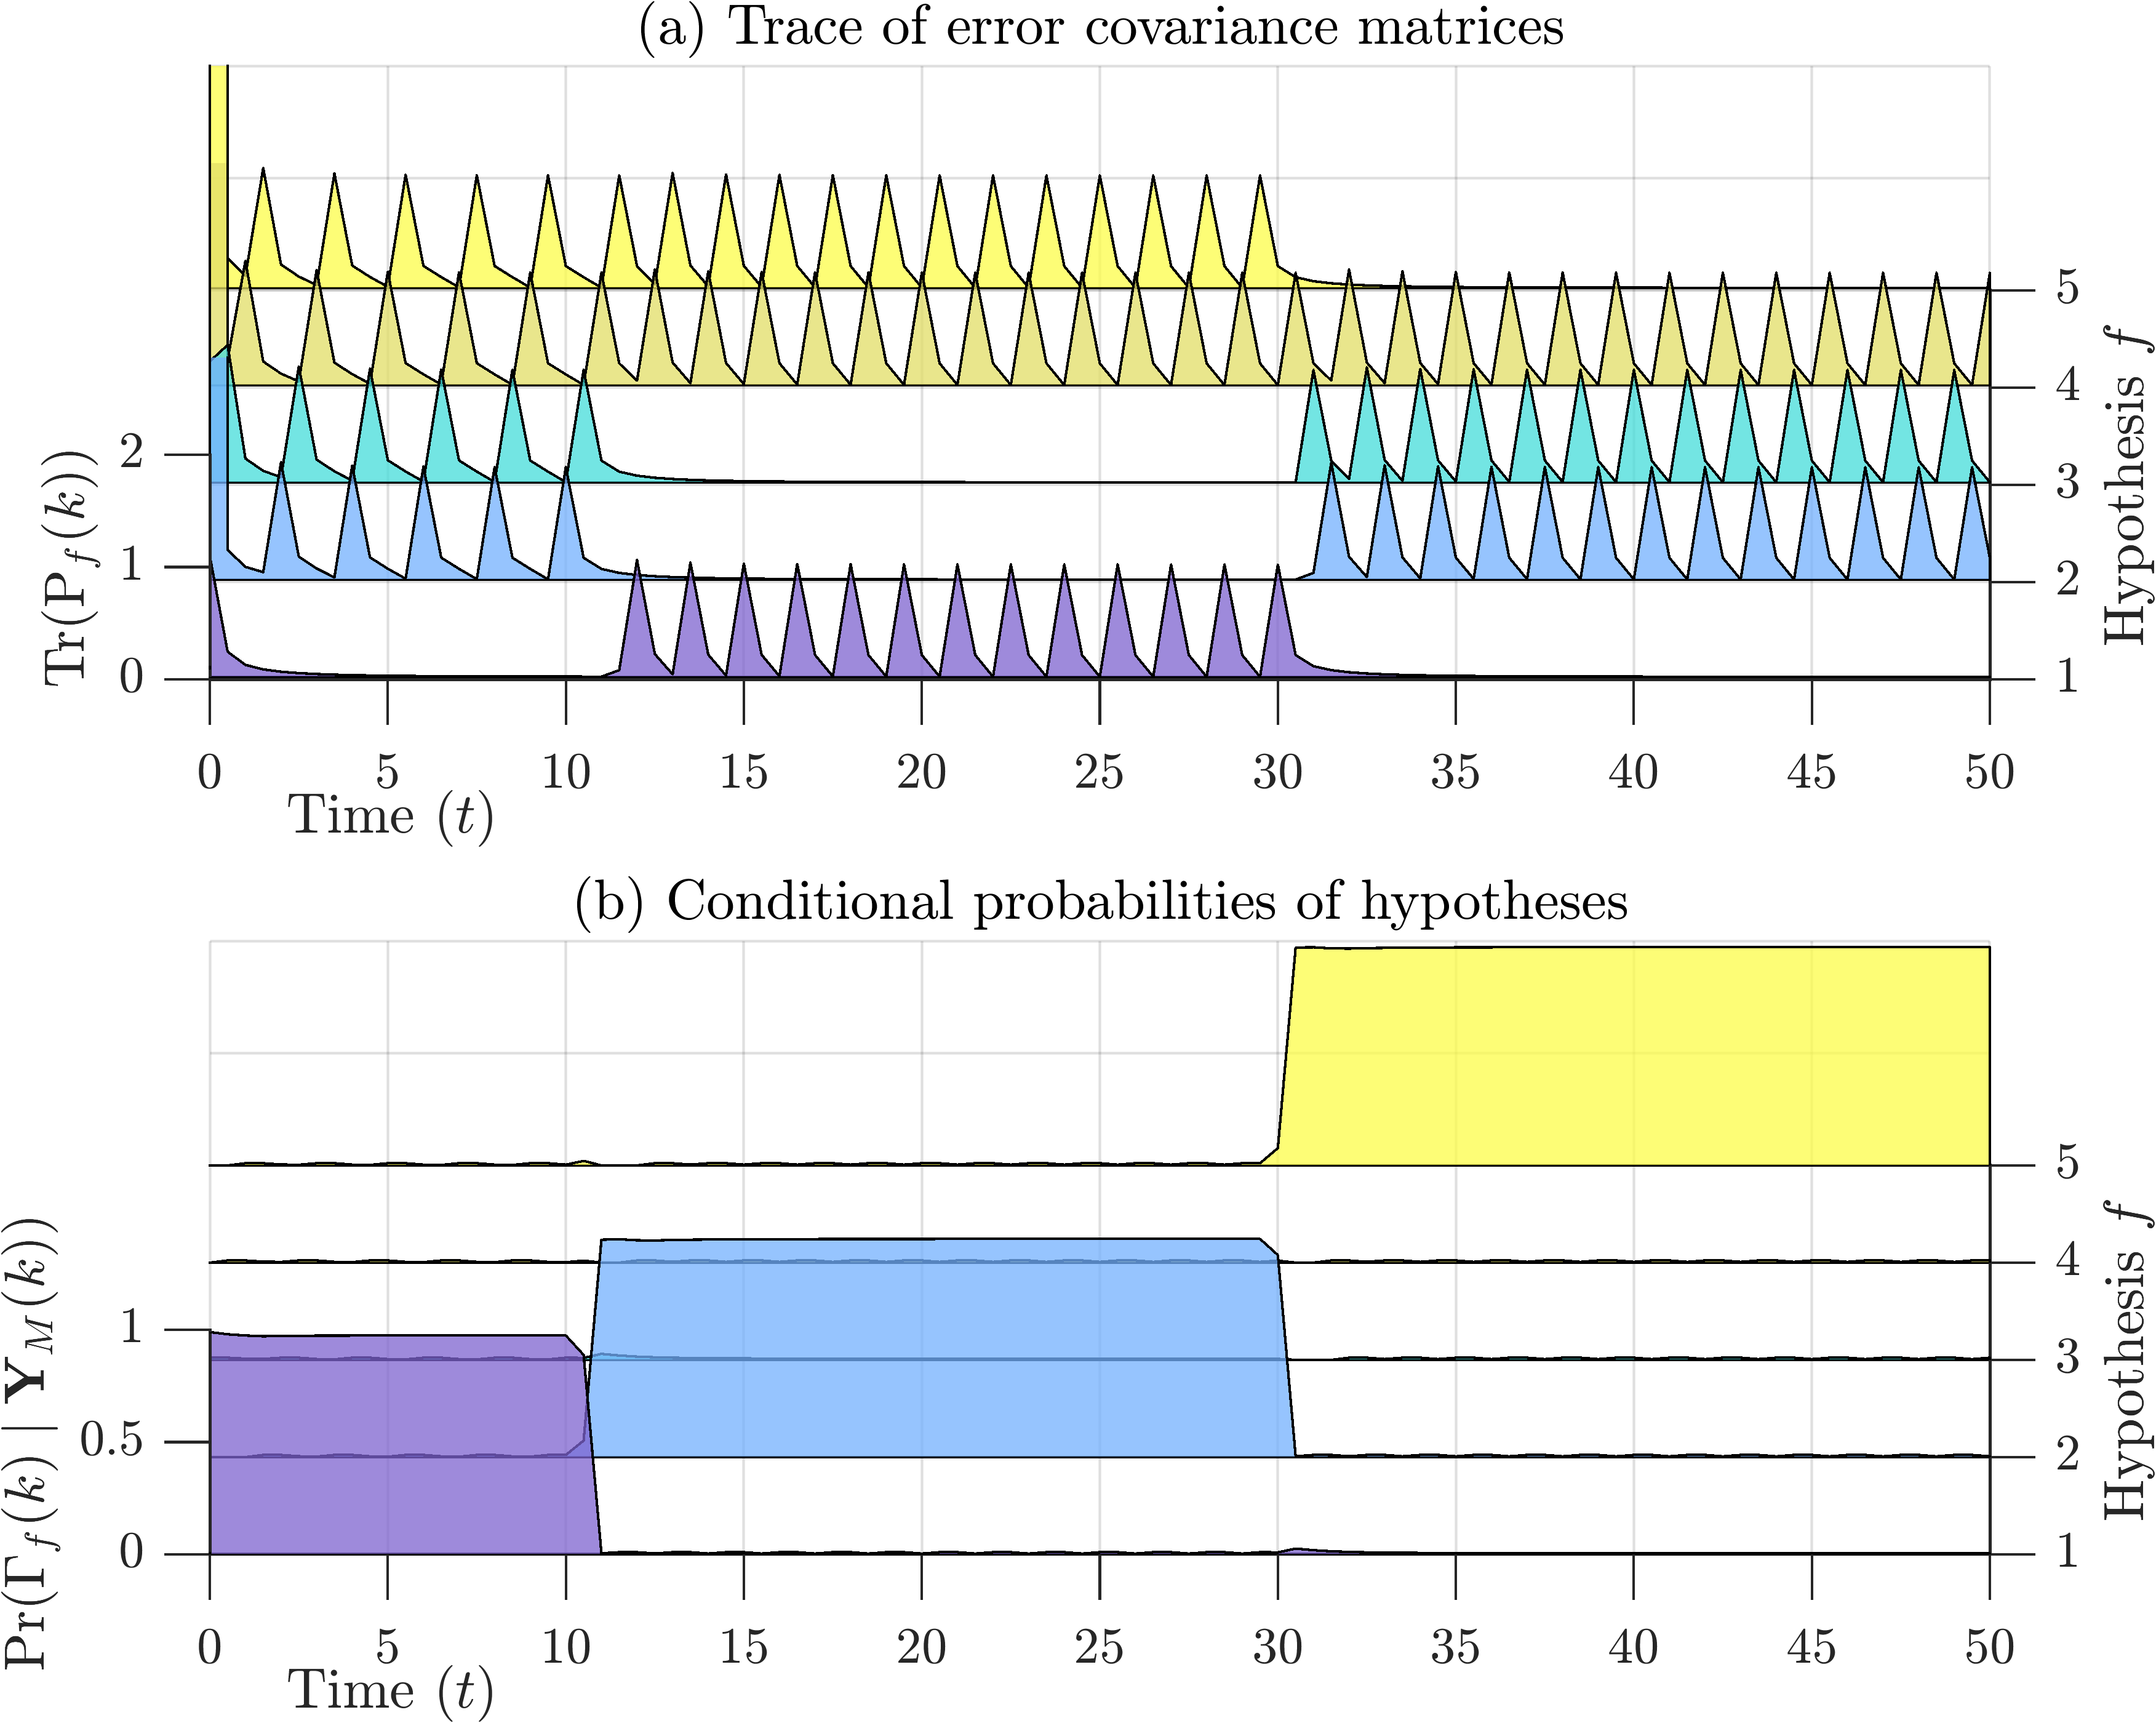
\includegraphics[width=12cm]{images/rod_MKF_test_sim_MKF_SP_prob.png}
	\caption{Multi-model observer probability estimates – MKF-SP}
	\label{fig:rod-obs-sim-test-probs-SP}
\end{figure}
\begin{figure}[htp]
	\centering
	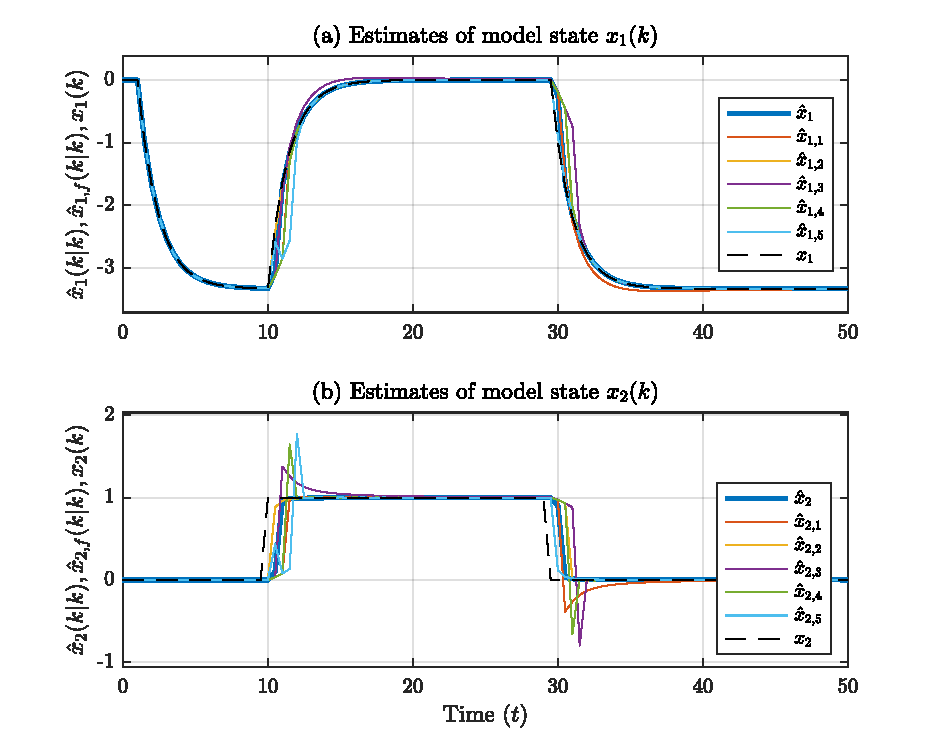
\includegraphics[width=13cm]{images/rod_MKF_test_sim_MKF_SP_x_est.pdf}
	\caption{Multi-model observer state estimates – MKF-SP}
	\label{fig:rod-obs-sim-test-x_est-SP}
\end{figure}
For comparison, Figures \ref{fig:rod-obs-sim-test-probs-SP} and \ref{fig:rod-obs-sim-test-x_est-SP} show the corresponding results of simulating the multi-model observer with the sequence pruning algorithm (labelled `MKF-SP') described by \cite{eriksson_classification_1996}, with $n_h=5$ and $n_{\text{min}}=2$. The plots for this simulation are more difficult to interpret than those of the sequence fusion observers because filters are continually pruned and cloned during the simulation. Therefore data presented as `filter $f$' in Figure \ref{fig:rod-obs-sim-test-probs-SP} do not come from the same Kalman filter at all times. Nevertheless, at each time instant there are 5 filters and the trace of their covariance matrices and conditional probabilities are shown. From these plots it can be seen that the hypotheses include many more possible shocks than those modelled by the sequence fusion observers. The estimates respond faster to the shock and the errors over the simulation period are lower than those of MKF-SF95 and MKF-SF98.

To evaluate and compare the performance of the observers, longer simulations with pseudo-random shock sequences and measurement noise were used. Figure \ref{fig:rod-obs-sim1-ioplot} shows the first 600 input-output data samples from a simulation of the system with a total duration of 2500 time units (5000 samples). The lower of the two plots shows the input signals, $u(k)$ and $p(k)$, from which it can be seen that two significant random shocks occurred during this period (at times $t=98$ and $220.5$). At other times, the value of $p(k)$ is a random walk due to the persistent component of the RODD disturbance (\ref{eq:wpk2}). In addition, a step change in $u(k)$ of magnitude 1 occurred at time $t=5$. The upper plot shows the simulated output measurements. The standard deviation of the measurement noise, $\sigma_M$, was $0.1$. No disturbances other than $w_p(k)$ were simulated (i.e. $w_1(k)=0$).

\subsubsection{Tuning of Kalman filters} \label{sim-obs-lin-1-KF-tuning}

\begin{figure}[htp]
	\centering
	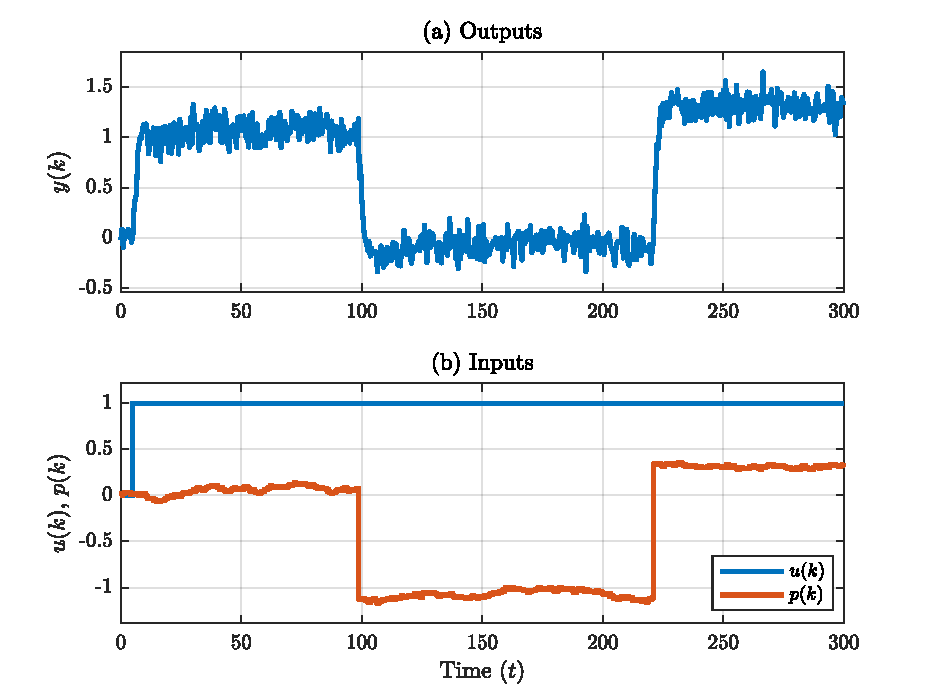
\includegraphics[width=13cm]{images/rod_obs_sim1_ioplot.pdf}
	\caption{Simulation of linear system with a RODD input disturbance}
	\label{fig:rod-obs-sim1-ioplot}
\end{figure}
Standard Kalman filters were used to develop a performance baselines with which to evaluate the sub-optimal multi-model observers. The question of how to set the gain of a Kalman filter when there is a RODD affecting the system is open to interpretation. One naive approach is to tune the Kalman filter using the variance of the persistent component of the disturbance, $\sigma_{w_p}^2$, if it is known. In this case, the Kalman filter, which is labelled `KF1', has a state disturbance covariance matrix
\begin{equation} \label{eq:sim-sys-siso-KF1-Q}
	\begin{aligned}
		\mathbf{Q}_{\text{KF1}}=\mathbf{Q}_0=\begin{bmatrix}
			\sigma_{x_1}^2 & 0 \\
			0 &  \sigma_{w_p}^2 \\
		\end{bmatrix}=\begin{bmatrix}
		0.01^2 & 0 \\
		0 & 0.01^2 \\
	\end{bmatrix}
	\end{aligned},
\end{equation}
where $\sigma_{x_1}^2$ is a parameter representing the variance of the errors of the process model state, $x_1$. However, this leads to a filter with a slow response to the shocks. It should be noted that the choice of $\sigma_{x_1}=0.01$ was somewhat arbitrary. In these simulations, the process is simulated by a model that is identical to the model used by the observers, so there is no model error in steady-state. However, during transient periods such as after a shock disturbance, errors between the observer model and the true states occur due to the delays in the system dynamics, and then the value of the process model error variance parameter $\sigma_{x_1}^2$ does have an effect.

A second option is to tune a Kalman filter to the variance of the shocks, $b^2\sigma_{w_p}^2$.  In this case, the Kalman filter, labelled `KF2', has a state disturbance covariance matrix
\begin{equation} \label{eq:sim-sys-siso-KF2-Q}
	\begin{aligned}
		\mathbf{Q}_{\text{KF2}}=\mathbf{Q}_1=\begin{bmatrix}
			\sigma_{x_1}^2 & 0 \\
			0 & b^2\sigma_{w_p}^2 \\
		\end{bmatrix}=\begin{bmatrix}
			0.01^2 & 0 \\
			0 & 1^2 \\
		\end{bmatrix}.
	\end{aligned}
\end{equation}

The problem with this filter is that it is very sensitive to the measurement noise, $v(k)$. 

As explained by \cite{robertson_detection_1995}, a trade off is needed. One approach to making this trade-off is to minimize the average estimation errors over a suitably long set of input-output data. In this case, 5000 samples were generated from the simulated system (Figure \ref{fig:sim-sys-diag-siso}) and then a Kalman filter was simulated multiple times, each time with a different tuning. Figure \ref{fig:sim-sys-siso-KF3-tuning} shows the results of these simulations, from which it can be seen that the lowest RMSEs were achieved when the variance parameter $\sigma_{w_p}^2$ was close to $0.01$. Using this result, a third Kalman filter labelled `KF3' was designed with the state disturbance covariance matrix 
\begin{equation} \label{eq:sim-sys-siso-KF3-Q}
	\begin{aligned}
		\mathbf{Q}_{\text{KF3}}=\mathbf{Q}_{\text{opt}}=\begin{bmatrix}
			\sigma_{x_1}^2 & 0 \\
			0 & \sigma_{w_p,\text{opt}}^2 \\
		\end{bmatrix}=\begin{bmatrix}
			0.01^2 & 0 \\
			0 & 0.1^2 \\
		\end{bmatrix}.
	\end{aligned}
\end{equation}

\begin{figure}[htp]
	\centering
	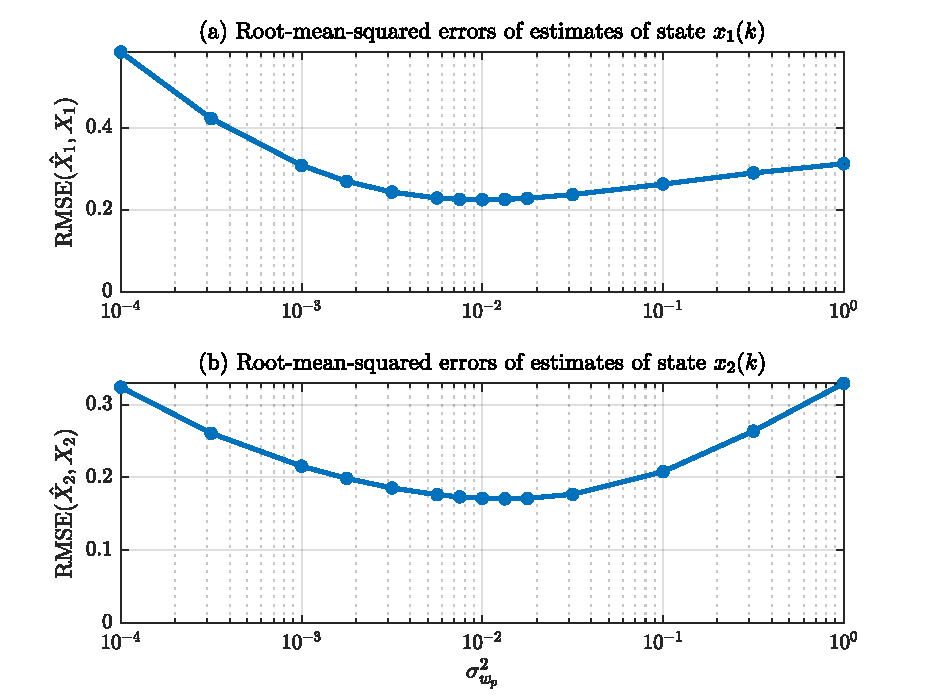
\includegraphics[width=13cm]{images/rod_obs_sim1_3KF_Q_seed_6.pdf}
	\caption{Tuning of Kalman filter KF3 – SISO system}
	\label{fig:sim-sys-siso-KF3-tuning}
\end{figure}
Figure \ref{fig:sim-sys-siso-KF123-est} shows the estimates of the three Kalman filters described above when simulated on the input-output data. The upper plot shows the output estimates and the lower plot shows the estimates of the second model state $x_{a,2}(k)$, which corresponds to the estimate of the RODD, $p(k)$. As expected, the response of KF1 to the infrequent step disturbances is noticeably slower than that of the other two. The response of KF2 is fast, but it is sensitive to the measurement noise. KF3 is a compromise between the two—a relatively fast response to the infrequent step changes and less sensitivity to the measurement noise.

\begin{figure}[htp]
	\centering
	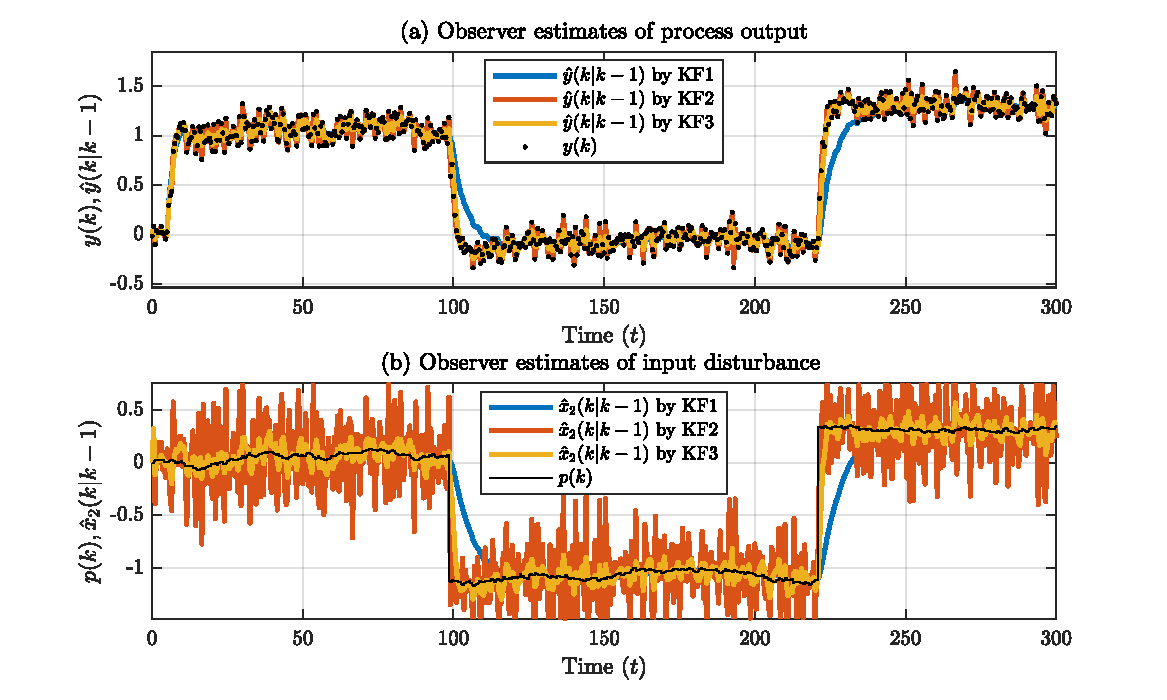
\includegraphics[width=13cm]{images/rod_obs_sim1_y_est1.pdf}
	\caption{Kalman filter estimates}
	\label{fig:sim-sys-siso-KF123-est}
\end{figure}
An alternative way to visualise the observer performance is to calculate the estimation errors by subtracting the estimates from the true values, which are known in these experiments. The upper plot in Figure \ref{fig:sim-sys-siso-KF123-cumerr} shows the errors in the output estimates of each Kalman filter when compared to the true process outputs (i.e. without measurement noise). The lower plot shows the cumulative sum of the squared errors. This clearly shows the differences in performance. The estimation errors of KF1 are small when the system is in steady-state but increase dramatically after each step disturbance. The magnitude of the errors of KF2 during steady-state periods is higher but roughly constant throughout the simulation. KF3 achieves the lowest overall cumulative sum-of-squared-errors by the end of the simulation.
\begin{figure}[htp]
	\centering
	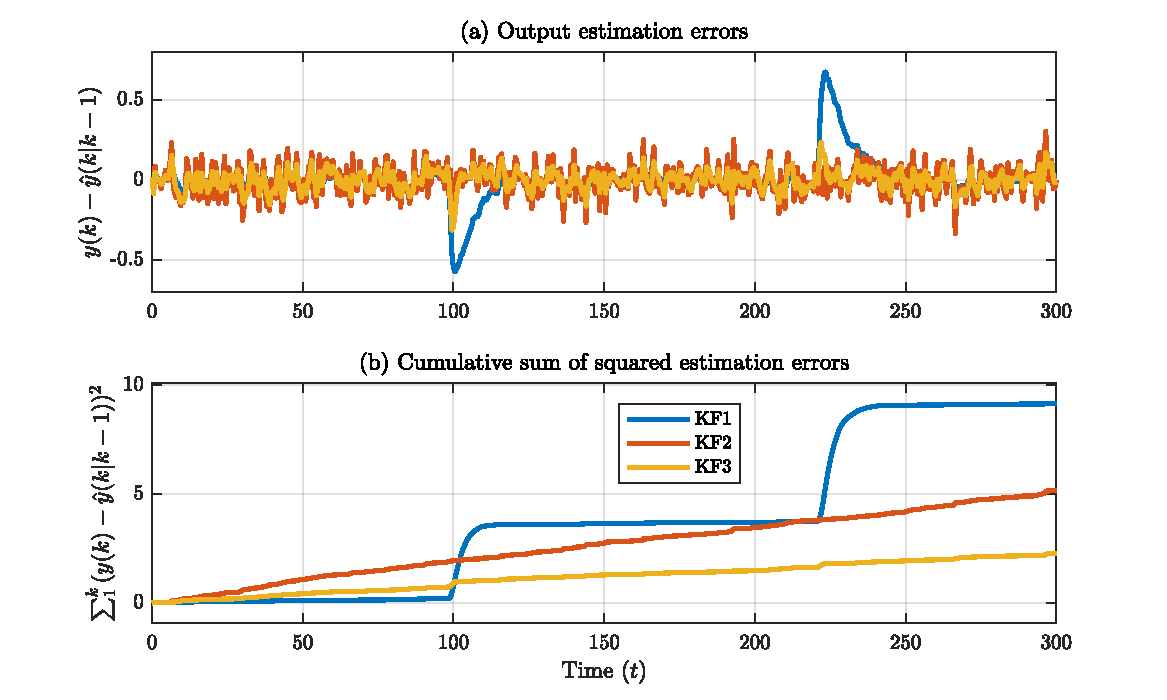
\includegraphics[width=13cm]{images/rod_obs_sim1_cum_err.pdf}
	\caption{Cumulative errors of Kalman filter estimates}
	\label{fig:sim-sys-siso-KF123-cumerr}
\end{figure}

\subsubsection{Selection of multi-model observer parameters} \label{sim-obs-lin-1-MKF-tuning}

Parameter values for the two sub-optimal multi-model observer algorithms described in Section \ref{subsec-fusion} were chosen by a similar method. The sequence fusion algorithm proposed by \cite{robertson_method_1998} has three parameters, $n_f$, $n_m$, and $n_d$. Candidate values for these parameters were generated by considering every combination satisfying

\begin{equation} \label{eq:sim-sys-siso-MKF-SF-param-values}
	\begin{aligned}
		\frac{n_f}{n_d} \in \left\{3, 5, 10, 15, 20\right\},  \\
		n_m \in \left\{1, 2, 3\right\},  \\
		n_d \in \left\{1, 2, 3, 5, 10\right\}.  \\
	\end{aligned}
\end{equation}

Note that $\frac{n_f}{n_d}$ represents the number of detection intervals within the fusion horizon and is always a whole number. Combinations were rejected when the number of hypotheses, $n_h$, was greater than 500 and when the total probability modelled (\ref{eq:p_gamma}) was less than 0.85. Each remaining combination was then evaluated by calculating the RMSE of the output estimates on the 5000 data samples from the simulated system. Table \ref{tb:obs-sim1-popt-SF98} shows the 10 best combinations of values evaluated (those with the lowest RMSE).

The sequence fusion algorithm evaluated in section \ref{section:sim-obs-lin} is based on \cite{robertson_method_1998}. However, Robertson and coworkers published results in 1995 \citep{robertson_detection_1995} using a slightly different version of this algorithm. Table \ref{tb:obs-sim1-popt-SF95} shows the results of a parameter search for the earlier version of the algorithm using the same simulation data used to tune the 1998 algorithm.

\begin{table}[hb]
	\begin{center}
		\caption{Multi-model observer parameter search results – MKF-SF95.} \label{tb:obs-sim1-popt-SF95}
		% See: https://texblog.org/2019/06/03/control-the-width-of-table-columns-tabular-in-latex/
		\begin{tabular}{p{0.05\textwidth}>{\centering\arraybackslash}p{0.07\textwidth}>{\centering\arraybackslash}p{0.07\textwidth}>{\centering\arraybackslash}p{0.07\textwidth}>{\centering\arraybackslash}p{0.07\textwidth}>{\centering\arraybackslash}p{0.24\textwidth}}
			$n_f$ & $n_m$ & $n_d$ & $n_h$ & $\beta$ & $\text{RMSE}(\hat{Y}(N),Y(N))$  \\
			\hline
			% Results with seed = 6, nT = 5000
			15 &   1 &   3 &   6 & 0.9035 & 0.1156 \\
			15 &   2 &   3 &  16 & 0.9044 & 0.1156 \\
			15 &   3 &   3 &  26 & 0.9044 & 0.1156 \\
			15 &   1 &   1 &  16 & 0.9904 & 0.1168 \\
			15 &   2 &   1 & 121 & 0.9996 & 0.1168 \\
			15 &   1 &   5 &   4 & 0.8861 & 0.1186 \\
			15 &   2 &   5 &   7 & 0.8864 & 0.1186 \\
			15 &   3 &   5 &   8 & 0.8864 & 0.1186 \\
			9 &   3 &   3 &   8 & 0.9415 & 0.1188 \\
			9 &   2 &   3 &   7 & 0.9415 & 0.1188 \\
			\hline
		\end{tabular}
	\end{center}
\end{table}

From these results it can be seen that the parameter tunings are quite similar to those in Table \ref{tb:obs-sim1-popt-SF98} for the 1998 variant of the algorithm. However, the best RMSE value achieved by the 1995 algorithm (0.1156) is slightly higher than the best achieved by the 1998 variant (0.1089) in this case.

Figure \ref{fig:rod-obs-sim1-yest-all-seed-RMSE-box-SF95} shows the results of both observers on different pseudo-random simulation results. This supports the finding by Robertson et al. that the 1998 variant of the algorithm performs better.

\begin{figure}[htp]
	\centering
	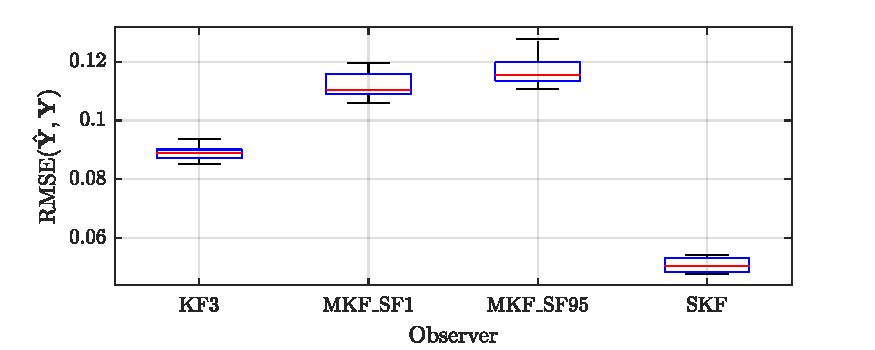
\includegraphics[width=12cm]{images/rod_obs_sim1_all_seed_y_err_box_SF95.pdf}
	\caption{Comparison of sequence fusion algorithm variants}
	\label{fig:rod-obs-sim1-yest-all-seed-RMSE-box-SF95}
\end{figure}

\begin{table}[hb]
	\begin{center}
		\caption{Multi-model observer parameter search results – MKF-SF95.} \label{tb:obs-sim1-popt-SF95}
		% See: https://texblog.org/2019/06/03/control-the-width-of-table-columns-tabular-in-latex/
		\begin{tabular}{p{0.05\textwidth}>{\centering\arraybackslash}p{0.07\textwidth}>{\centering\arraybackslash}p{0.07\textwidth}>{\centering\arraybackslash}p{0.07\textwidth}>{\centering\arraybackslash}p{0.07\textwidth}>{\centering\arraybackslash}p{0.24\textwidth}}
			$n_f$ & $n_m$ & $n_d$ & $n_h$ & $\beta$ & $\text{RMSE}(\hat{Y}(N),Y(N))$  \\
			\hline
			% Results with seed = 6, after fixing MKF-SF98
			15 &   1 &   1 &  16 & 0.9904 & 0.1168 \\
			15 &   2 &   1 & 121 & 0.9996 & 0.1168 \\
			9 &   1 &   3 &   4 & 0.9412 & 0.1180 \\
			9 &   2 &   3 &   7 & 0.9415 & 0.1180 \\
			9 &   3 &   3 &   8 & 0.9415 & 0.1180 \\
			15 &   1 &   3 &   6 & 0.9035 & 0.1186 \\
			15 &   2 &   3 &  16 & 0.9044 & 0.1186 \\
			15 &   3 &   3 &  26 & 0.9044 & 0.1186 \\
			15 &   1 &   5 &   4 & 0.8861 & 0.1207 \\
			15 &   2 &   5 &   7 & 0.8864 & 0.1207 \\
			\hline
		\end{tabular}
	\end{center}
\end{table}

\begin{table}[hb]
	\begin{center}
		\caption{Multi-model observer parameter search results – MKF-SF98.} \label{tb:obs-sim1-popt-SF98}
		% See: https://texblog.org/2019/06/03/control-the-width-of-table-columns-tabular-in-latex/
		\begin{tabular}{p{0.05\textwidth}>{\centering\arraybackslash}p{0.07\textwidth}>{\centering\arraybackslash}p{0.07\textwidth}>{\centering\arraybackslash}p{0.07\textwidth}>{\centering\arraybackslash}p{0.07\textwidth}>{\centering\arraybackslash}p{0.24\textwidth}}
			$n_f$ & $n_m$ & $n_d$ & $n_h$ & $\beta$ & $\text{RMSE}(\hat{Y}(N),Y(N))$  \\
			\hline
			% Results with seed = 6
			%15 &   1 &   5 &   4 & 0.9930 & 0.1089 \\
			%15 &   2 &   5 &   7 & 0.9999 & 0.1089 \\
			%15 &   3 &   5 &   8 & 1.0000 & 0.1089 \\
			%15 &   1 &   3 &   6 & 0.9917 & 0.1118 \\
			%15 &   2 &   3 &  16 & 0.9997 & 0.1118 \\
			%15 &   3 &   3 &  26 & 1.0000 & 0.1118 \\
			%15 &   1 &   1 &  16 & 0.9904 & 0.1168 \\
			%15 &   2 &   1 & 121 & 0.9996 & 0.1168 \\
			%10 &   1 &   1 &  11 & 0.9957 & 0.1219 \\
			%10 &   2 &   1 &  56 & 0.9999 & 0.1219 \\
			% Results with seed = 6, after fixing MKF_SF98
			15 &   1 &   1 &  16 & 0.9904 & 0.1168 \\
			15 &   2 &   1 & 121 & 0.9996 & 0.1168 \\
			10 &   1 &   1 &  11 & 0.9957 & 0.1219 \\
			10 &   2 &   1 &  56 & 0.9999 & 0.1219 \\
			10 &   3 &   1 & 176 & 1.0000 & 0.1219 \\
			15 &   1 &   3 &   6 & 0.9917 & 0.1235 \\
			15 &   2 &   3 &  16 & 0.9997 & 0.1235 \\
			15 &   3 &   3 &  26 & 1.0000 & 0.1235 \\
			10 &   1 &   2 &   6 & 0.9962 & 0.1290 \\
			10 &   2 &   2 &  16 & 0.9999 & 0.1290 \\
			\hline
		\end{tabular}
	\end{center}
\end{table}

A fusion horizon of $n_f=15$ sample periods produced the best results. For this horizon length, the lowest errors were produced when the length of the detection interval was 5 sample periods ($n_d=5$). Increasing the maximum possible number of shocks during the fusion horizon ($n_m$) had no significant benefit and increases the number of hypotheses to be modelled ($n_h$).

It is noteworthy that a combination requiring only 4 filters produced a better result than all others. Two combinations of parameter values were selected for further evaluation. Firstly, the best combination, $n_f=15$, $n_{min}=1$, and $n_d=5$, which is used in the observer labelled `MKF-SF1', and a second, labelled `MKF-SF2', with parameter values $n_f=15$, $n_{min}=2$, and $n_d=3$.

The sequence pruning algorithm proposed by \cite{eriksson_classification_1996} has two parameters to be specified, $n_h$, and $n_{min}$. Candidate values for these parameters were generated by considering all combinations satisfying

\begin{equation} \label{eq:sim-sys-siso-MKF-SP-param-values}
	\begin{aligned}
		n_h \in \left\{3, 4, 5, 7, 10, 14, 19, 25, 32\right\},  \\
			n_{min} \in \left\{1, 2, 3, 4, 5, 6, 7, 9, 12, 16, 21\right\}.  \\
		\end{aligned}
	\end{equation}

Combinations where rejected when $n_h - n_{min} < 1$, or in other words, when the minimum life $n_{min}$ was greater than or equal to the number of hypotheses, $n_h$. This is a necessary condition because there must be enough filters to simulate the hypotheses until they are pruned. Each remaining combination was then evaluated by calculating the RMSE of the output estimates of the observer on the same 5000 samples used in the tuning of the MKF-SF1 observer, as described above. Table \ref{tb:obs-sim1-popt-SP} shows the 10 combinations of parameter values which produced the lowest RMSE on the same 5000 sample dataset used for the sequence fusion parameter search.

\begin{table}[hb]
	\begin{center}
		\caption{Multi-model observer parameter search results – MKF-SP.} \label{tb:obs-sim1-popt-SP}
		% See: https://texblog.org/2019/06/03/control-the-width-of-table-columns-tabular-in-latex/
		\begin{tabular}{p{0.05\textwidth}>{\centering\arraybackslash}p{0.07\textwidth}>{\centering\arraybackslash}p{0.24\textwidth}}
			$n_h$ & $n_\text{min}$ & $\text{RMSE}(\hat{Y}(N),Y(N))$  \\
			\hline
			% Results with seed = 6, nT = 5000
			10 &   7 & 0.0576  \\
			10 &   6 & 0.0577  \\
			14 &  12 & 0.0577  \\
			19 &  16 & 0.0577  \\
			25 &  21 & 0.0577  \\
			14 &   7 & 0.0577  \\
			19 &   7 & 0.0578  \\
			25 &  16 & 0.0578  \\
			19 &   6 & 0.0578  \\
			25 &  12 & 0.0578  \\
			\hline
		\end{tabular}
	\end{center}
\end{table}

%		   % seed = 0, nT = 2500
%			  7 &   3 & 0.0569  \\
%			10 &   8 & 0.0570  \\
%			14 &  12 & 0.0570  \\
%			25 &  22 & 0.0570  \\
%			10 &   3 & 0.0570  \\
%			20 &  17 & 0.0570  \\
%			14 &   3 & 0.0570  \\
%			14 &   4 & 0.0570  \\
%			14 &   8 & 0.0571  \\
%			50 &  44 & 0.0571  \\
%			% seed = 2, nT = 2500
%			  7 &   3 & 0.0608  \\
%			19 &  16 & 0.0608  \\
%			14 &  12 & 0.0608  \\
%			25 &  21 & 0.0609  \\
%			10 &   5 & 0.0609  \\
%			10 &   6 & 0.0609  \\
%			10 &   4 & 0.0609  \\
%			  7 &   2 & 0.0609  \\
%			10 &   3 & 0.0609  \\
%			14 &   4 & 0.0609  \\


In this case, the differences between the RMSEs of the best 10 combinations are very small, indicating that the choice of parameters from these combinations was not critical. The combination $n_h=10$ and $n_{min}=7$ was chosen for the observer which is labelled `MKF-SP1'. It should also be noted that the best RMSEs of this observer are significantly lower than those of the best sequence fusion observer in Table \ref{tb:obs-sim1-popt-SF95}. The parameters for all the observers used in the simulations in this section are summarised in Table \ref{tb:obs-params-sim1}.

\begin{table}[hb]
	\begin{center}
		\caption{Observers and parameters for SISO linear system.} \label{tb:obs-params-sim1}
		% See: https://texblog.org/2019/06/03/control-the-width-of-table-columns-tabular-in-latex/
		\begin{tabular}{p{0.16\textwidth}>{\centering\arraybackslash}p{0.1\textwidth}>{\centering\arraybackslash}p{0.16\textwidth}>{\centering\arraybackslash}p{0.16\textwidth}>{\centering\arraybackslash}p{0.16\textwidth}}
			& KF3 & MKF-SF95 & MKF-SF98 & MKF-SP \\
			\hline
			Type & Kalman filter & Multi-model Kalman filter & Multi-model Kalman filter & Multi-model Kalman filter \\
			Sub-optimal algorithm & - & Sequence fusion & Sequence fusion & Sequence pruning \\
			\hline
			Parameters &  &  &  &  \\
			$\mathbf{Q}$ & $\mathbf{Q}_{opt}$ & $\{\mathbf{Q}_0,\mathbf{Q}_1\}$ & $\{\mathbf{Q}_0,\mathbf{Q}'_1\}$ & $\{\mathbf{Q}_0,\mathbf{Q}_1\}$ \\
			$R$ & $0.1^2$ & $0.1^2$ & $0.1^2$ & $0.1^2$ \\
			$\mathbf{P}(0)$ & $\mathbf{P}_0$ & $\mathbf{P}_0$ & $\mathbf{P}_0$ & $\mathbf{P}_0$ \\
			No. of filters & 1 & 4 & 16 & 7 \\
			$n_f$ & - & 15 & 15 & - \\
			$n_m$ & - & 1 & 2 & - \\
			$n_d$ & - & 5 & 3 & - \\
			$n_{min}$ & - & - & - & 4 \\
			$\epsilon$ & - & 0.01 & 0.01 & 0.01 \\
			$\sigma_{w_p}$ & - & 0.01 & 0.01 & 0.01 \\
			$b$ & - & 100 & 100 & 100 \\
			\hline
		\end{tabular}
	\end{center}
\end{table}

\subsubsection{Scheduled Kalman filter} \label{sim-obs-lin-1-SKF}

To understand the maximum performance that could be achieved by an ideal multi-model observer, a hypothetical observer that has access to the true shock indicator signal $\gamma(k)$ was simulated. This `scheduled' Kalman filter, labelled ‘SKF’, has only one shock sequence---the correct one---and therefore the process noise covariance is automatically scheduled to match the known shock signal. The SKF is hypothetical because it cannot be implemented in reality since the random shocks are not measured.

\subsubsection{Stochastic simulation results} \label{sim-obs-lin-1-results}

Figure \ref{fig:rod-obs-sim1-yest-1-SF} shows the estimates of the two sequence fusion observers, MKF-SF1 and MKF-SF2, compared to the optimally-tuned Kalman filter, KF3, and the scheduled Kalman Filter, SKF, over the first 300 time units of the simulation. Figure \ref{fig:rod-obs-sim1-yest-2-SF} is a closer look at the same results in the vicinity of the first step disturbance, which occurs at $t=98$.
\begin{figure}[htp]
	\centering
	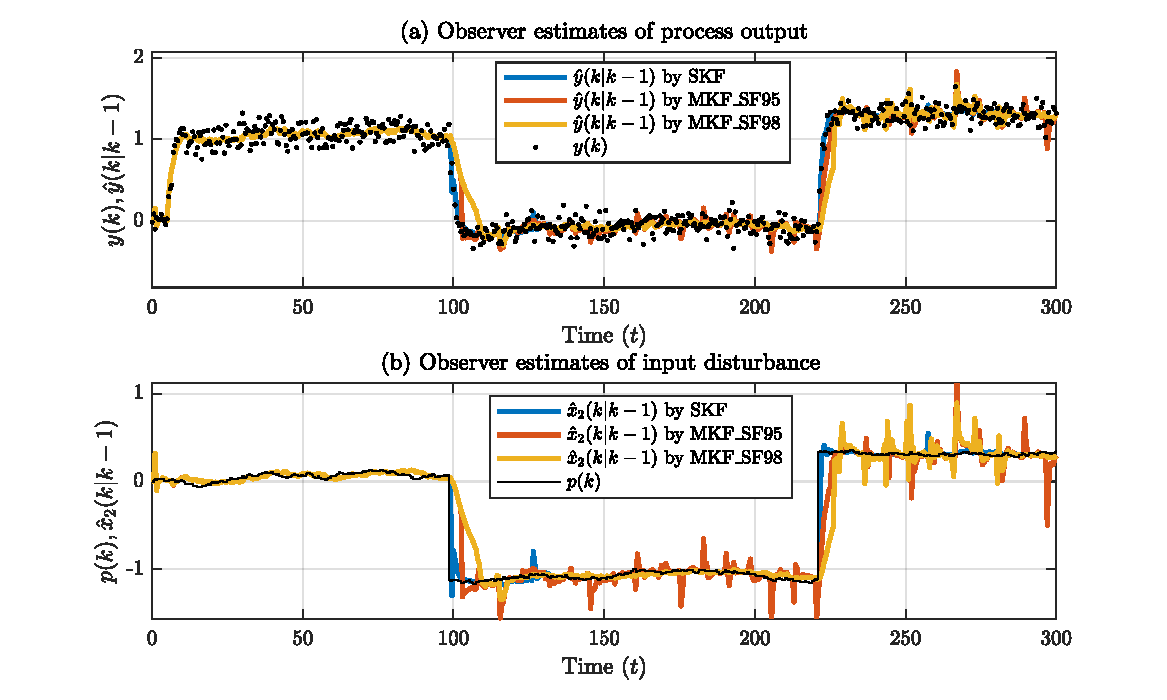
\includegraphics[width=13cm]{images/rod_obs_sim1_all_seed_y_est1_SF95_SF98.pdf}
	\caption{Estimates by sequence fusion observer – SISO system}
	\label{fig:rod-obs-sim1-yest-1-SF}
\end{figure}

% Not enough space for this detailed plot
%\begin{figure}[htp]
%	\centering
%	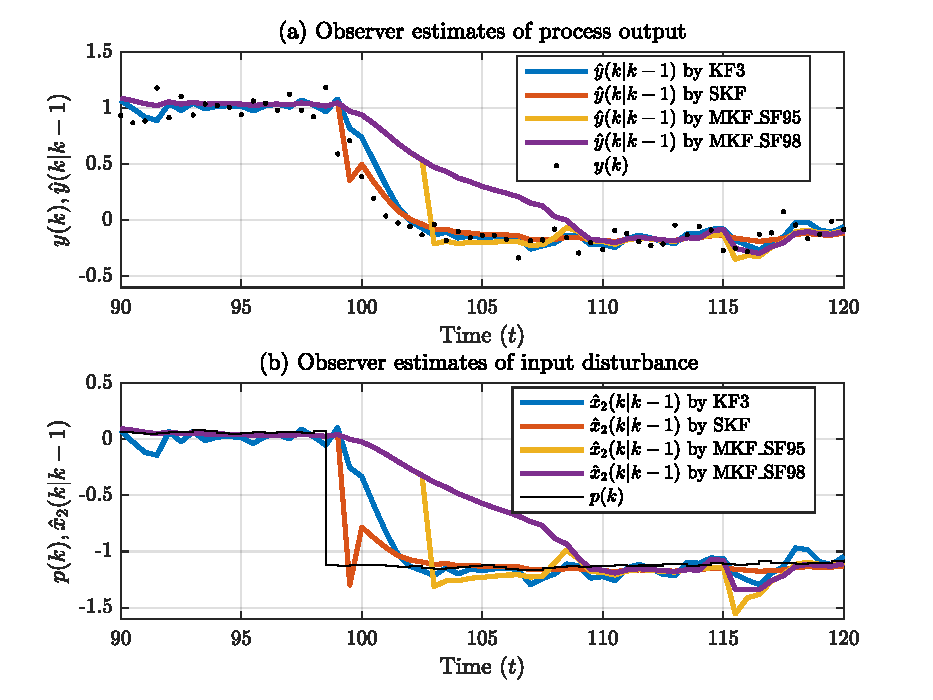
\includegraphics[width=13cm]{images/rod_obs_sim1_all_seed_y_est2_SF95_SF98.pdf}
%	\caption{Estimates by sequence fusion observer – SISO system}
%	\label{fig:rod-obs-sim1-yest-2-SF}
%\end{figure}

A number of observations can be made about these results. Firstly, prior to the occurrence of the first shock, the variation in the estimates of the multi-model observers is lower than that of KF3 (i.e. the estimates are less sensitive to the measurement noise) and about as good as the SKF. Secondly, the response of both the multi-model observers to the occurrence of the first shock is slow and delayed compared to the others. Thirdly, after the first shock, the variance of MKF-SF1 and MKF-SF2 is higher than that of KF3.

Figures \ref{fig:rod-obs-sim1-yest-1-SP} and \ref{fig:rod-obs-sim1-yest-2-SP} show the estimates of the sequence pruning observer, MKF-SP1, compared to the optimally-tuned Kalman filter, KF3, and the scheduled Kalman Filter, SKF.  From these results, it can be seen that the sequence pruning observer is less sensitive to the measurement noise before and after the shocks. It also responds very quickly to the shock occurrence, almost as fast as the SKF, which represents the best possible performance of any multi-model observer.
\begin{figure}[htp]
	\centering
	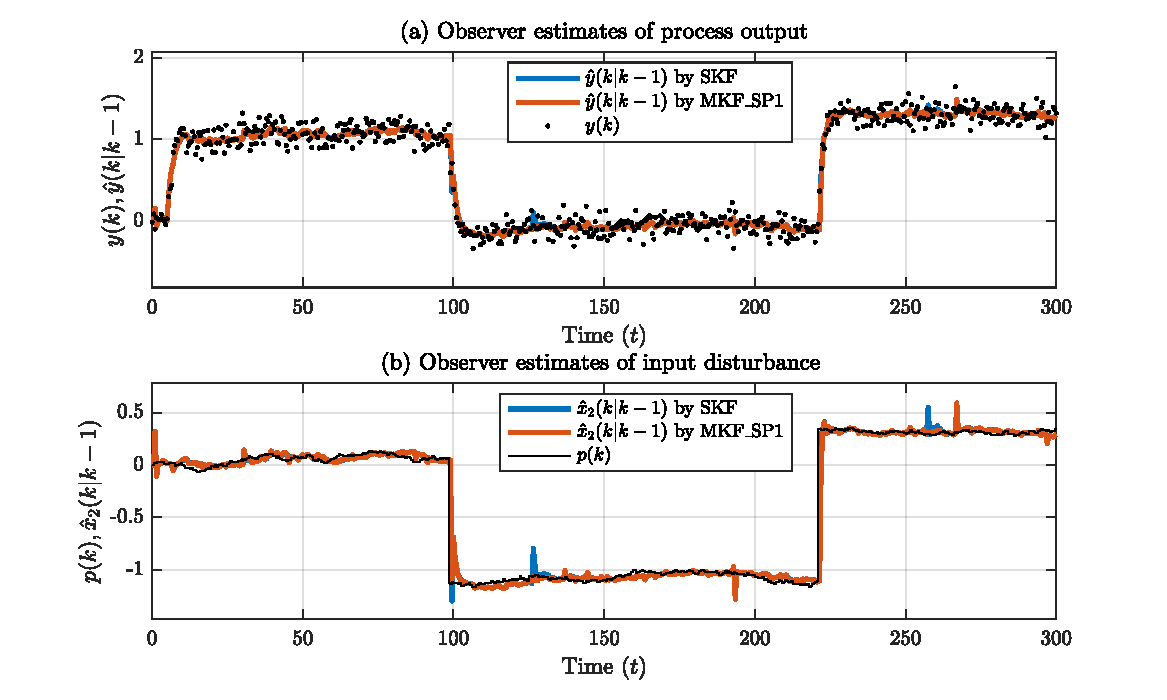
\includegraphics[width=13cm]{images/rod_obs_sim1_all_seed_y_est1_SP1.pdf}
	\caption{Estimates by sequence pruning observer – SISO system}
	\label{fig:rod-obs-sim1-yest-1-SP}
\end{figure}

% Not enough space for this detailed plot
%\begin{figure}[htp]
%	\centering
%	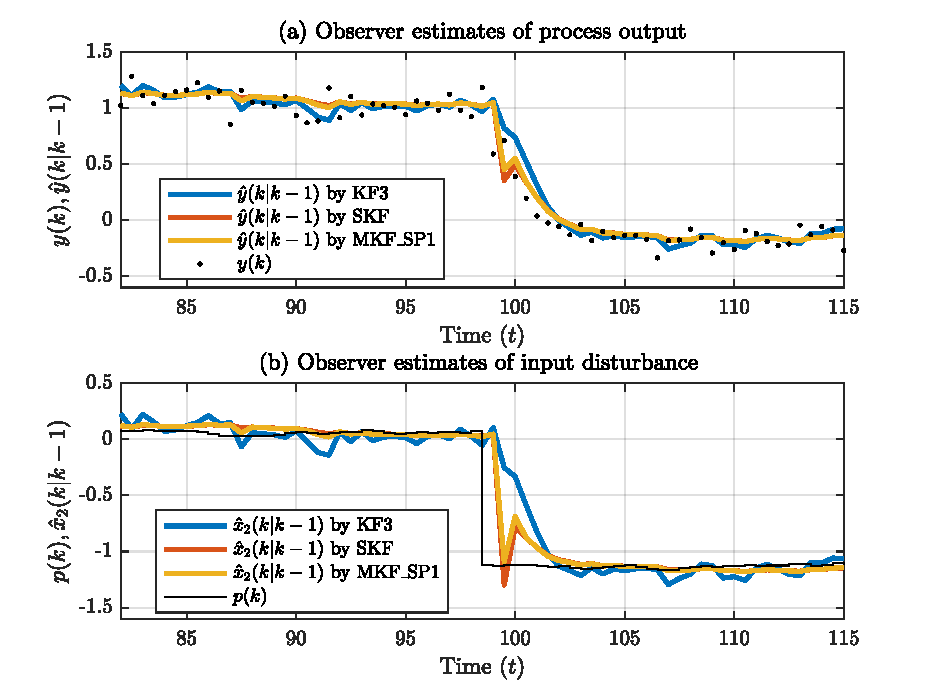
\includegraphics[width=13cm]{images/rod_obs_sim1_all_seed_y_est2_SP1.pdf}
%	\caption{Estimates by sequence pruning observer – SISO system}
%	\label{fig:rod-obs-sim1-yest-2-SP}
%\end{figure}
\begin{figure}[htp]
	\centering
	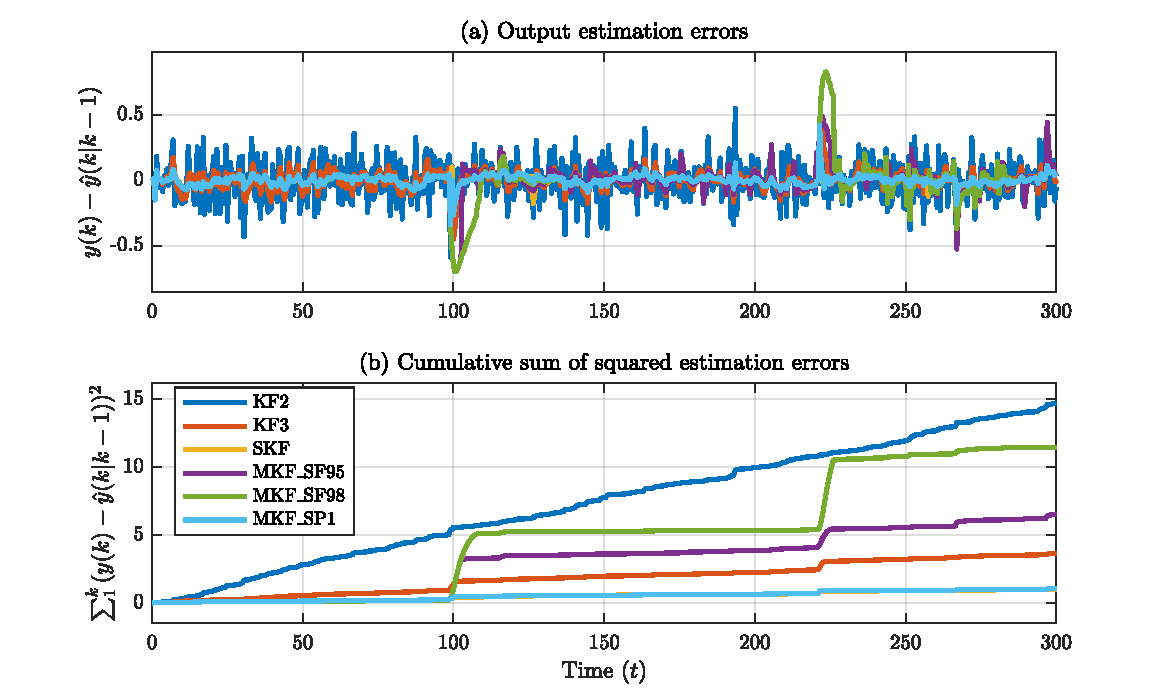
\includegraphics[width=13cm]{images/rod_obs_sim1_all_seed_cum_err_y1.pdf}
	\caption{Cumulative errors of observer estimates – SISO system}
	\label{fig:rod-obs-sim1-cum-err-y1-all}
\end{figure}
Figure \ref{fig:rod-obs-sim1-xest-RMSE-bar} compares the RMSEs of the state estimates of the five observers over the full length of the simulation, which was 2500 time units, or 5000 sample periods in length.
\begin{figure}[htp]
	\centering
	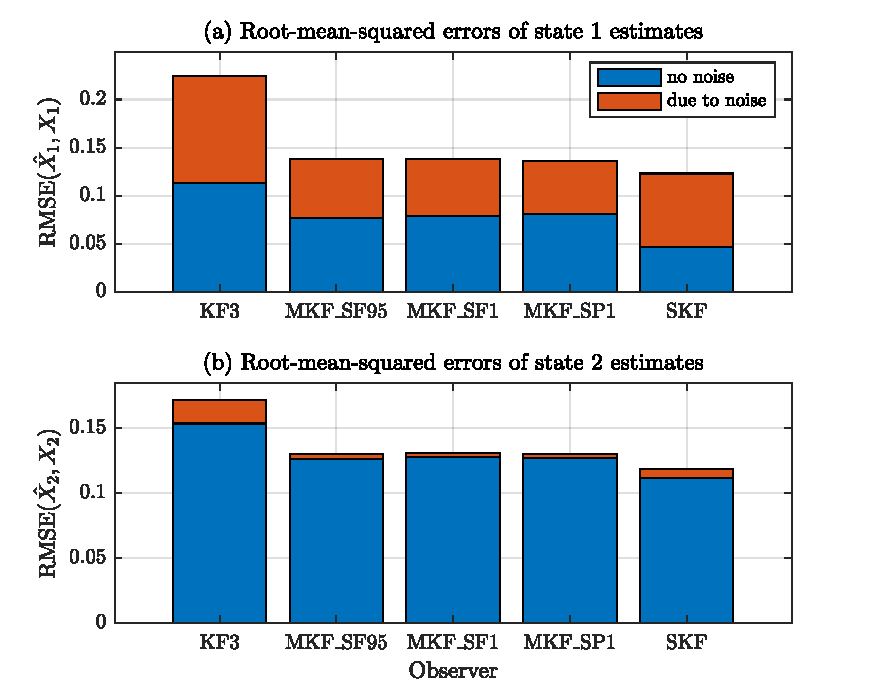
\includegraphics[width=12cm]{images/rod_obs_sim1_all_seed_x_err_bar.pdf}
	\caption{Root-mean-squared errors of state estimates – SISO system}
	\label{fig:rod-obs-sim1-xest-RMSE-bar}
\end{figure}

Because these processes are stochastic, it is important to run simulations of sufficient duration to be confident that the results are representative of the expected performance of the observers. Figure \ref{fig:rod-obs-sim1-yest-all-seed-RMSE-box} provides an indication of the sensitivity of the RMSE values to the initialization of the pseudo-random number generator used in these simulations. This figure shows the results of 10 simulations of 5000 samples each, carried out with different initializations. From these results it can be seen that the RMSE values are somewhat sensitive to the random initialization but that the differences between the three observers are significant enough and highly unlikely to be a result of the random initialization. Therefore, these simulations of duration 5000 sample periods may be considered sufficient for the purposes of evaluating the relative performance of these observers.
\begin{figure}[htp]
	\centering
	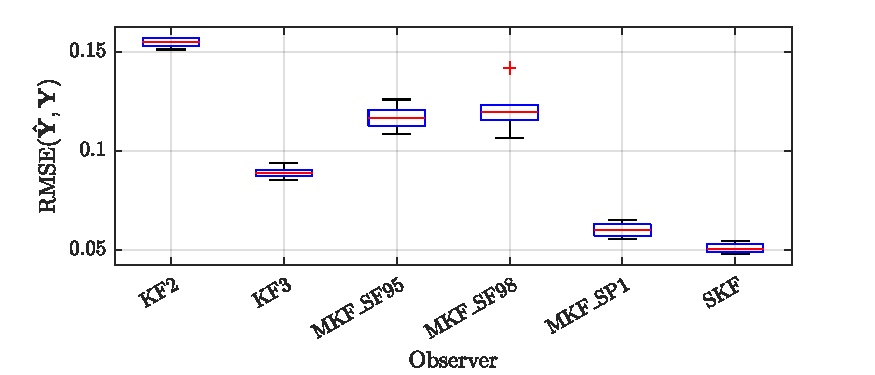
\includegraphics[width=12cm]{images/rod_obs_sim1_all_seed_y_err_box.pdf}
	\caption{Sensitivity of output estimates to random initialization – SISO system}
	\label{fig:rod-obs-sim1-yest-all-seed-RMSE-box}
\end{figure}

From these results, it was concluded that the multi-model observer proposed by \cite{robertson_method_1998} was not a good state estimator for this SISO system with one RODD step disturbance. The sequence pruning algorithm proposed by \cite{eriksson_classification_1996}, on the other hand, seems to be a very good state estimator, significantly better than a single, well tuned Kalman filter.

% Plots for analysis of SF performance
%
%\begin{figure}[htp]
%	\centering
%	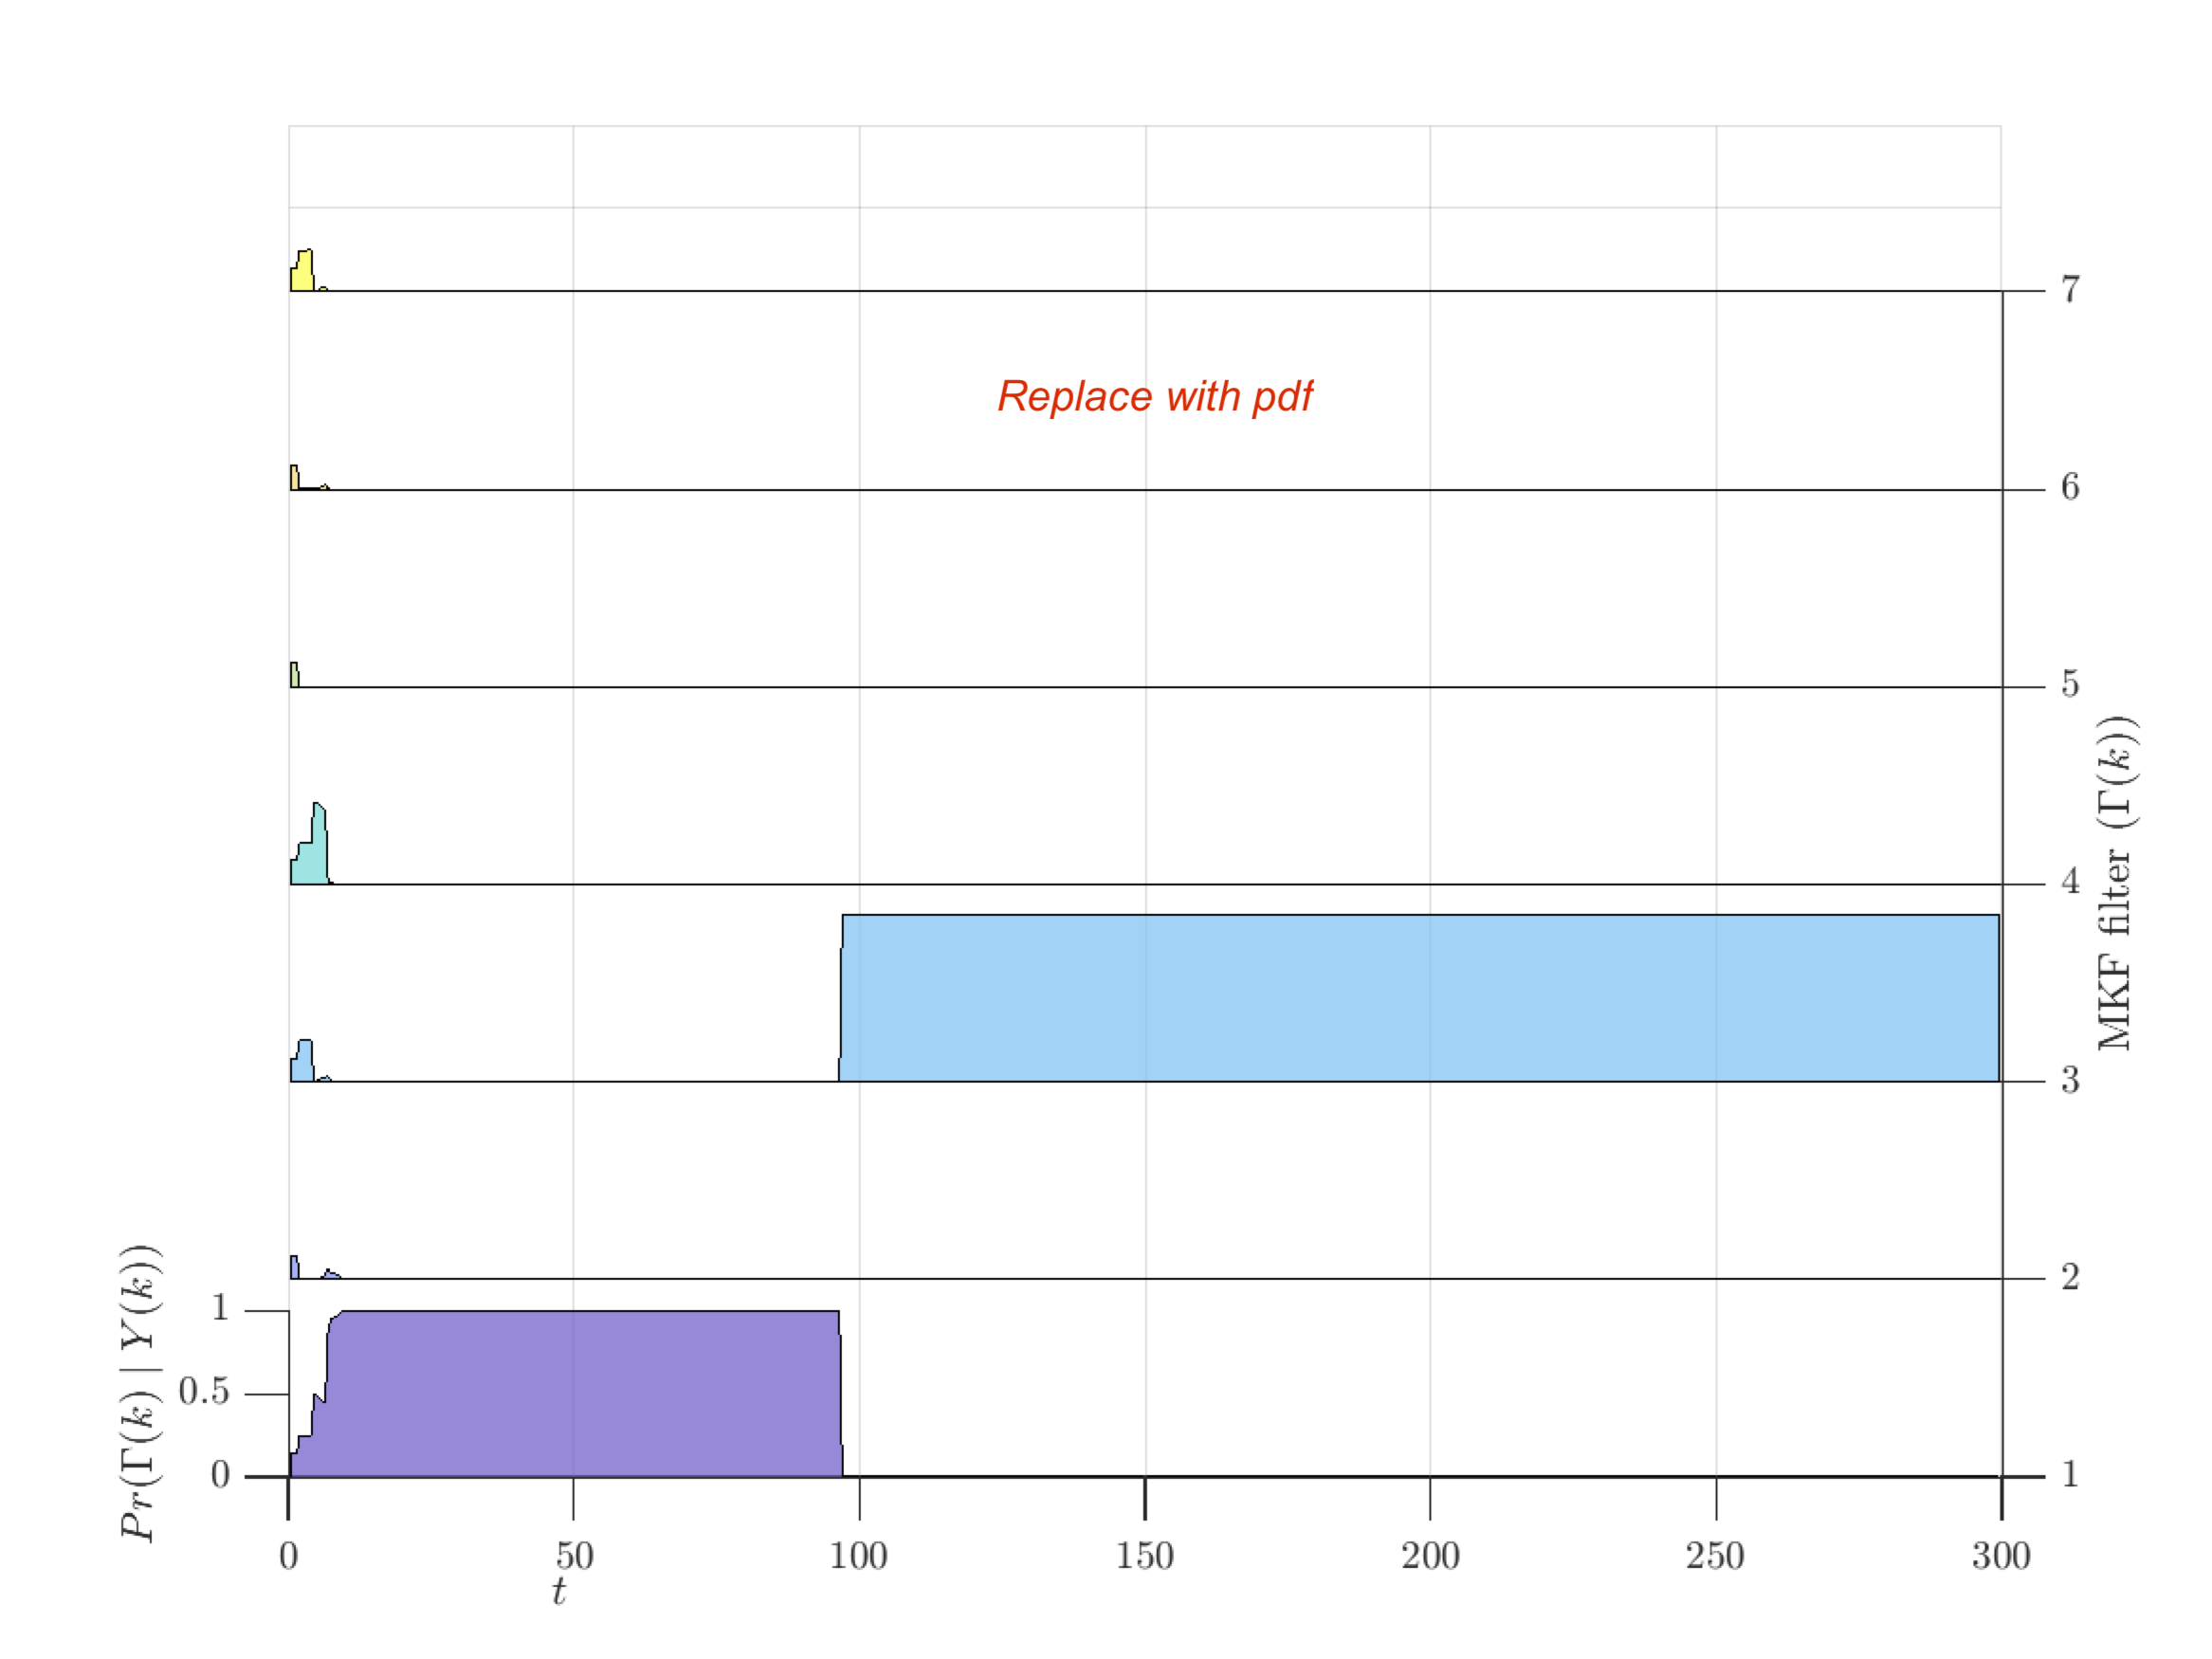
\includegraphics[width=15cm]{images/rod-obs-sim-1-4-wfplot-DRAFT.png}
%	\caption{Evolution of conditional probabilities with sequence fusion}
%	\label{fig:rod-obs-sim1-4-wfplot}
%\end{figure}
%
%\begin{figure}[htp]
%	\centering
%	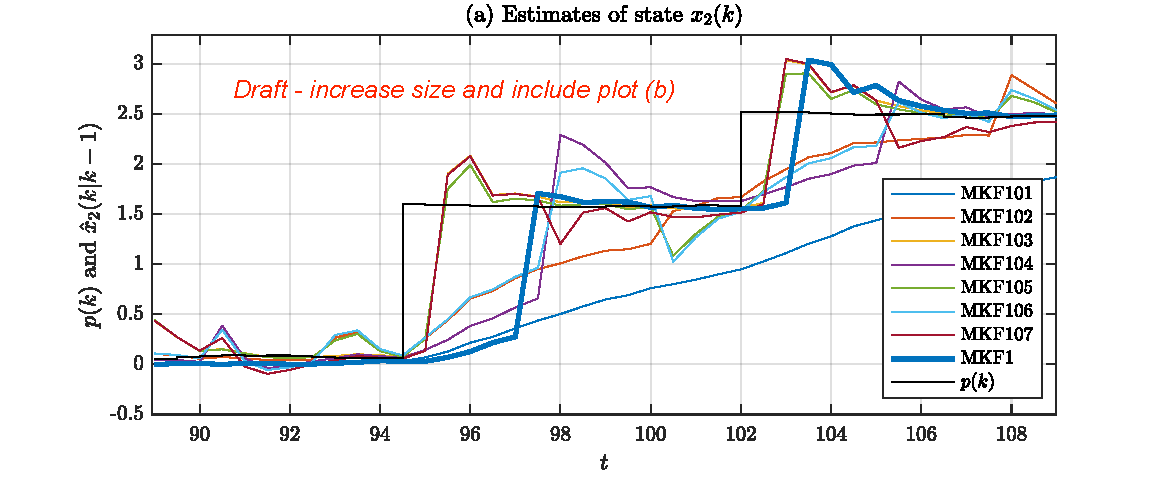
\includegraphics[width=14cm]{images/rod-obs-sim-1-4-est-MKF-SF-plot-DRAFT.pdf}
%	\caption{Filter estimates of sequence fusion observer during step disturbances}
%	\label{fig:rod-obs-sim1-4-est-MKF-SF-plot-DRAFT}
%\end{figure}
%
%\begin{figure}[htp]
%	\centering
%	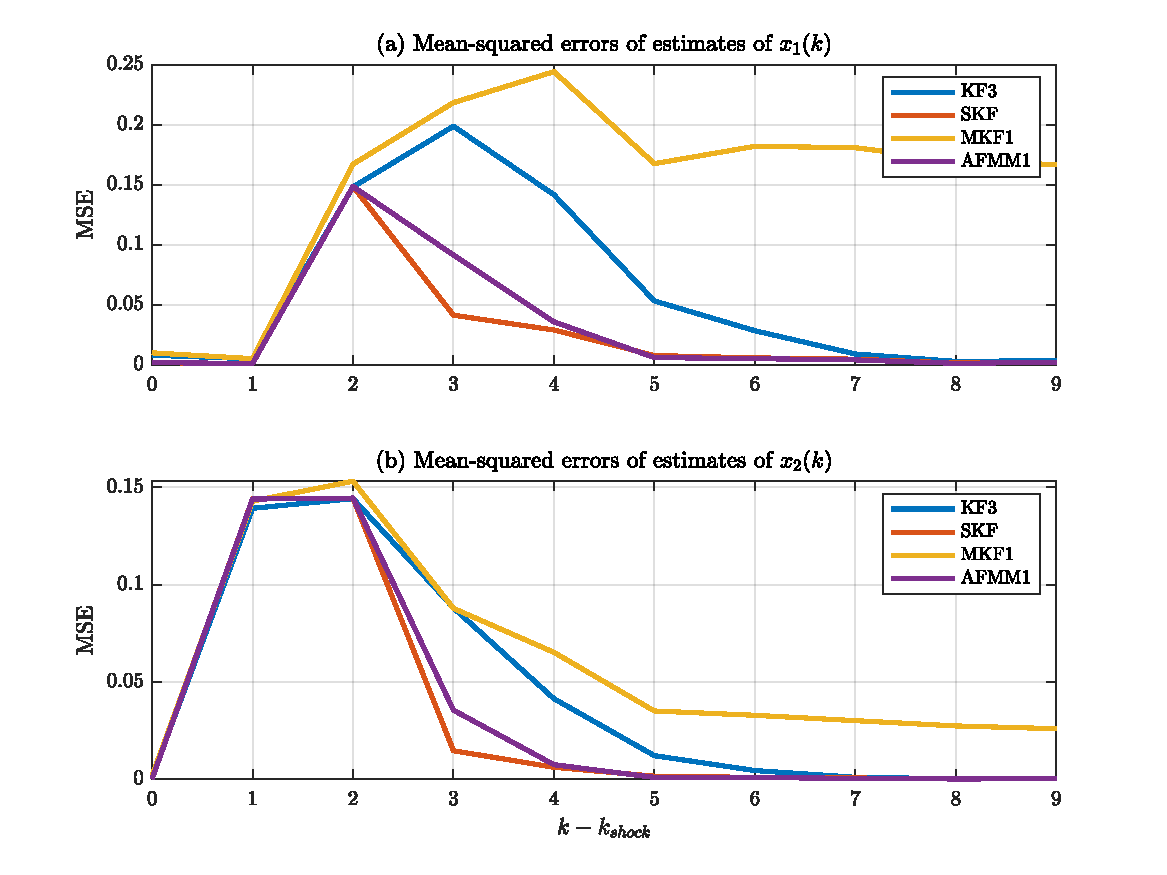
\includegraphics[width=14cm]{images/rod_obs_sim2_7_mse_ashocks.pdf}
%	\caption{Average errors of observer estimates after shock disturbances}
%	\label{fig:rod_obs_sim2_7_mse_ashocks}
%\end{figure}

\subsection{MIMO linear system} \label{sim-obs-lin-2}

To investigate the performance of the observers in estimating the states of a \textit{multiple-input, multiple output} (MIMO) system, a 2-input, 2-output ($2\times2$) process model was chosen, with two independent RODD step disturbance, one added to each manipulatable input, as shown in the functional diagram in Figure \ref{fig:sim-sys-diag-2x2}. 

The model used to simulate the process is a discrete-time linear model derived from the continuous-time system,
\begin{equation} \label{eq:sim-sys-siso--ct}
	\mathbf{G}_p(s) = \left[\begin{array}{cc}
		G_{11}(s) & G_{12}(s)  \\
		G_{21}(s) & G_{22}(s)  \\
	\end{array}\right] = \left[\begin{array}{cc}
		\frac{1}{1+8.5s} & \frac{-0.5}{1+8.5s}  \\
		\frac{-0.5}{1+8.5s} & \frac{1}{1+8.5s}  \\
	\end{array}\right]
\end{equation}
where $s$ is the Laplace variable.  This was converted to a discrete-time model with a sampling period of $T=1$. The discrete-time state space representation used to simulate the augmented system including disturbances was
\begin{equation} \label{eq:sim-sys-2x2-ss-aug}
	\begin{split}
		\mathbf{x}_{a}(k+1) & =\left[\begin{array}{cccc}
			0.8890 & 0 & 1 & -0.5 \\
			0 & 0.8890 & -0.5 & 1 \\
			0 & 0 & 1 & 0 \\
			0 & 0 & 0 & 1
		\end{array}\right] \mathbf{x}_{a}(k) + \left[\begin{array}{cc}
			1 & -0.5 \\
			-0.5 & 1
		\end{array}\right] \mathbf{u}(k) + \mathbf{w}_{a}(k) \\
		y(k) & =\left[\begin{array}{cccc}
			0.1110 & 0 & 0 & 0 \\
			0 & 0.1110 & 0 & 0
		\end{array}\right] \mathbf{x}_{a}(k) + v(k)
	\end{split}
\end{equation}
where
\begin{equation} \label{eq:sim-sys-2x2-ss-aug2}
	\mathbf{x}_{a}(k) = \left[\begin{array}{l}
		x_{1}(k) \\
		x_{2}(k) \\
		p_{1}(k) \\
		p_{2}(k)
	\end{array}\right], \mathbf{w}_{a}(k) = \left[\begin{array}{l}
		w_1(k) \\
		w_2(k) \\
		w_{p,1}(k) \\
		w_{p,2}(k)
	\end{array}\right].
\end{equation}

Figure \ref{fig:rod-obs-sim-2-ioplot} shows a set of  300 input-output  data samples generated by simulating this system for a duration of 300 time units. The lower of the two plots shows the input signals, $u_1(k)$, $u_2(k)$, $p_1(k)$, and $p_2(k)$. From this it can be seen that 3 random shocks occurred of various magnitudes and that $p_1(k)$ and $p_2(k)$ are random walks in between the shocks. In this case, there were no changes to the known input variables, $u_1(k)$, and $u_2(k)$. The upper plot shows the simulated output measurements, $y_1(k)$ and $y_2(k)$. The standard deviation of the measurement noises, $\sigma_{M,1}$ and $\sigma_{M,2}$, were both $0.1$. No input disturbances other than $w_{p,1}(k)$ and $w_{p,2}(k)$ were simulated (i.e. $w_1(k)=w_2(k)=0$).

As in the previous experiment, a standard Kalman filter was tuned experimentally to achieve a low RMSE of the output estimates.  The details of this tuning process are included in Annex \ref{section:annex-sim-2-KF-tuning}. 

\begin{figure}[htp]
	\centering
	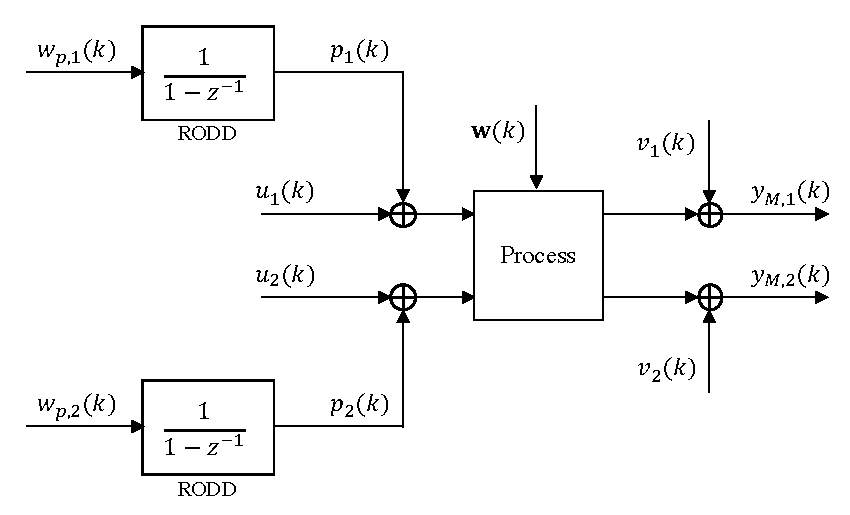
\includegraphics[width=11.5cm]{images/sim-sys-diag-2x2.pdf}
	\caption{Functional diagram of the simulated MIMO system}
	\label{fig:sim-sys-diag-2x2}
\end{figure}

\begin{itemize}
	\item Best KF tuning $\sigma_{w_p}^2=0.0075$
\end{itemize}

\begin{figure}[htp]
	\centering
	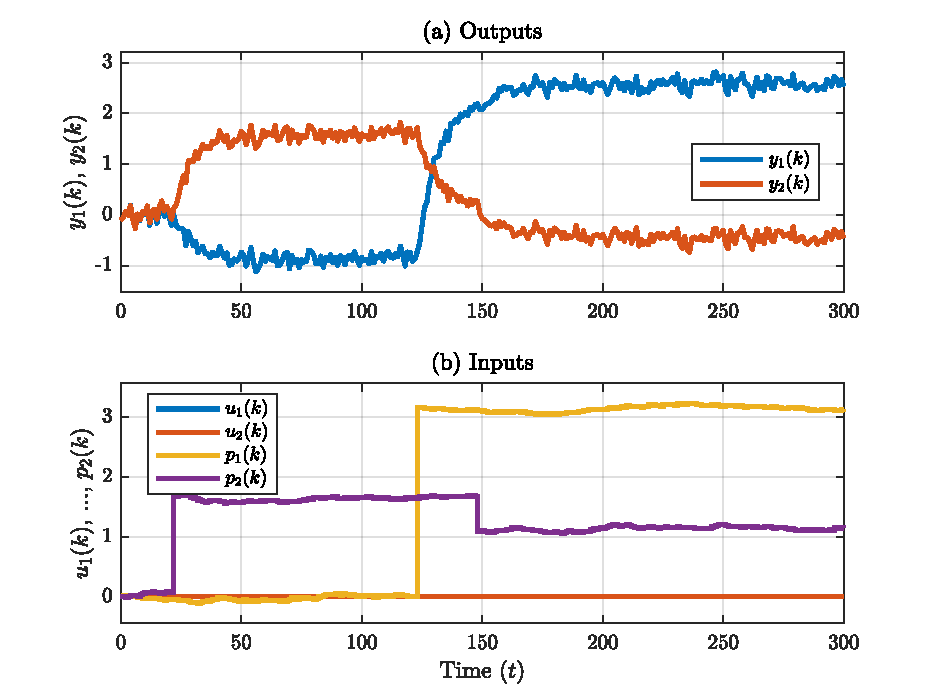
\includegraphics[width=13cm]{images/rod_obs_sim2_ioplot.pdf}
	\caption{Simulation of linear MIMO system with two RODDs}
	\label{fig:rod-obs-sim-2-ioplot}
\end{figure}

\begin{figure}[htp]
	\centering
	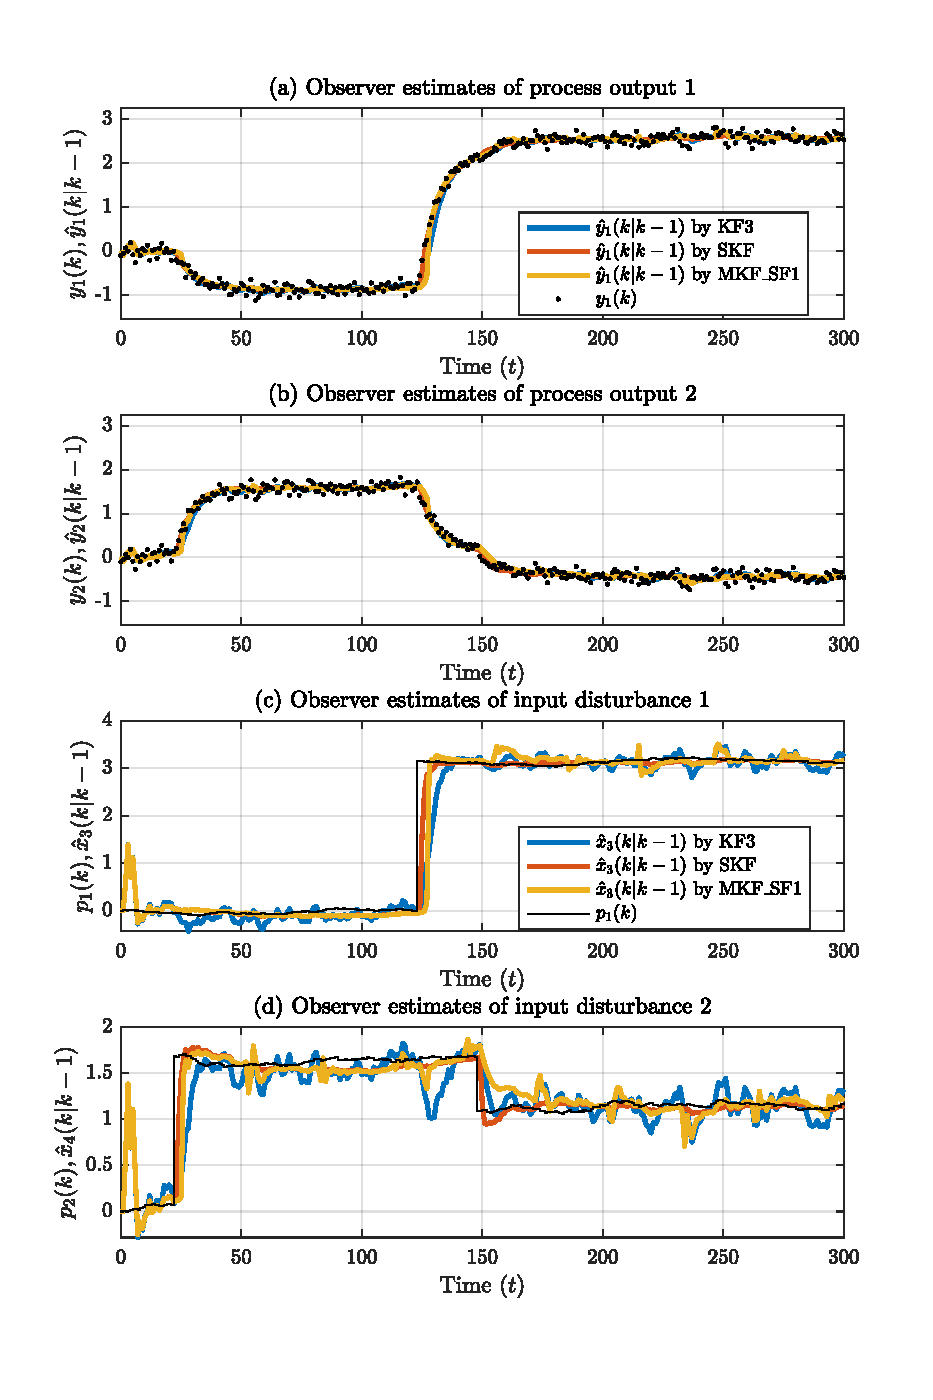
\includegraphics[width=13cm]{images/rod_obs_sim2_all_seed_y_est1_SF1.pdf}
	\caption{Estimates by sequence fusion observer –  $2\times2$ system}
	\label{fig:rod-obs-sim2-yest-1-SF}
\end{figure}

\begin{figure}[htp]
	\centering
	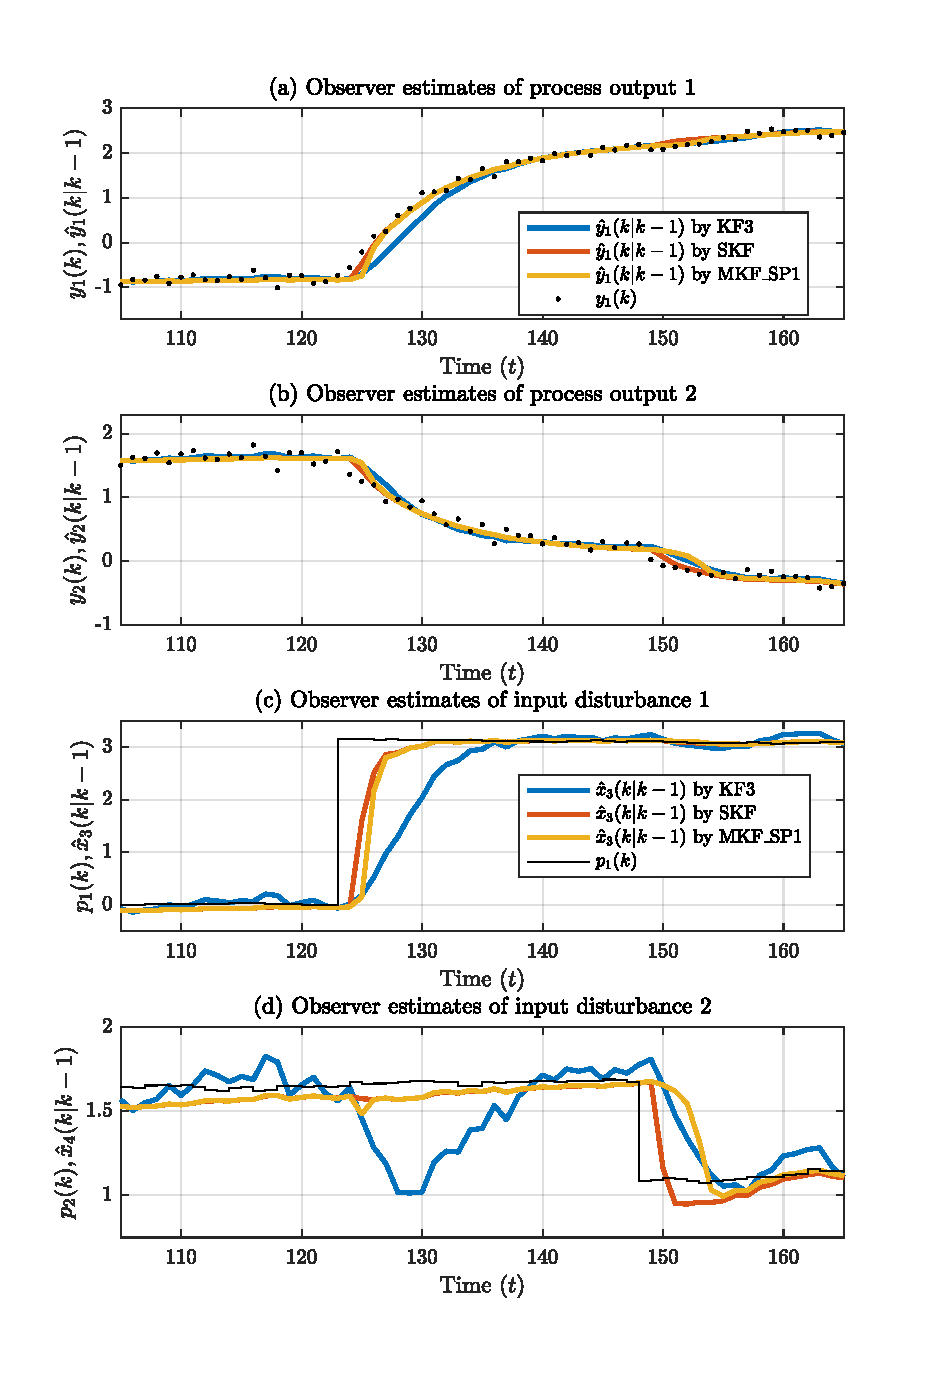
\includegraphics[width=13cm]{images/rod_obs_sim2_all_seed_y_est2_SP1.pdf}
	\caption{Estimates by sequence pruning observer –  $2\times2$ system}
	\label{fig:rod-obs-sim2-yest-2-SF}
\end{figure}

\begin{figure}[htp]
	\centering
	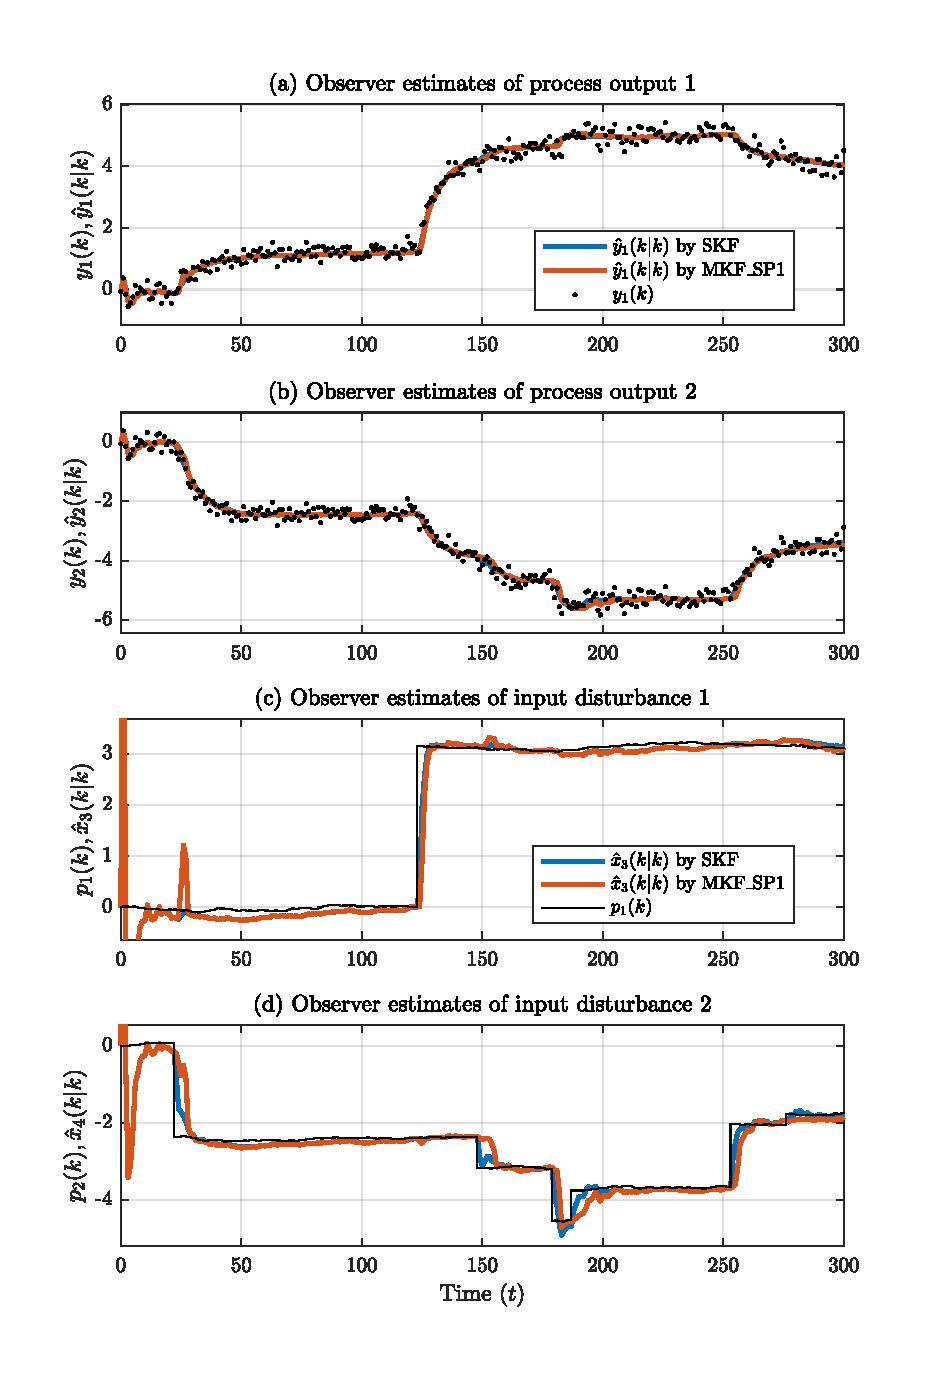
\includegraphics[width=13cm]{images/rod_obs_sim2_all_seed_y_est1_SP1.pdf}
	\caption{Estimates by sequence pruning observer –  $2\times2$ system}
	\label{fig:rod-obs-sim2-yest-1-SP}
\end{figure}

\begin{figure}[htp]
	\centering
	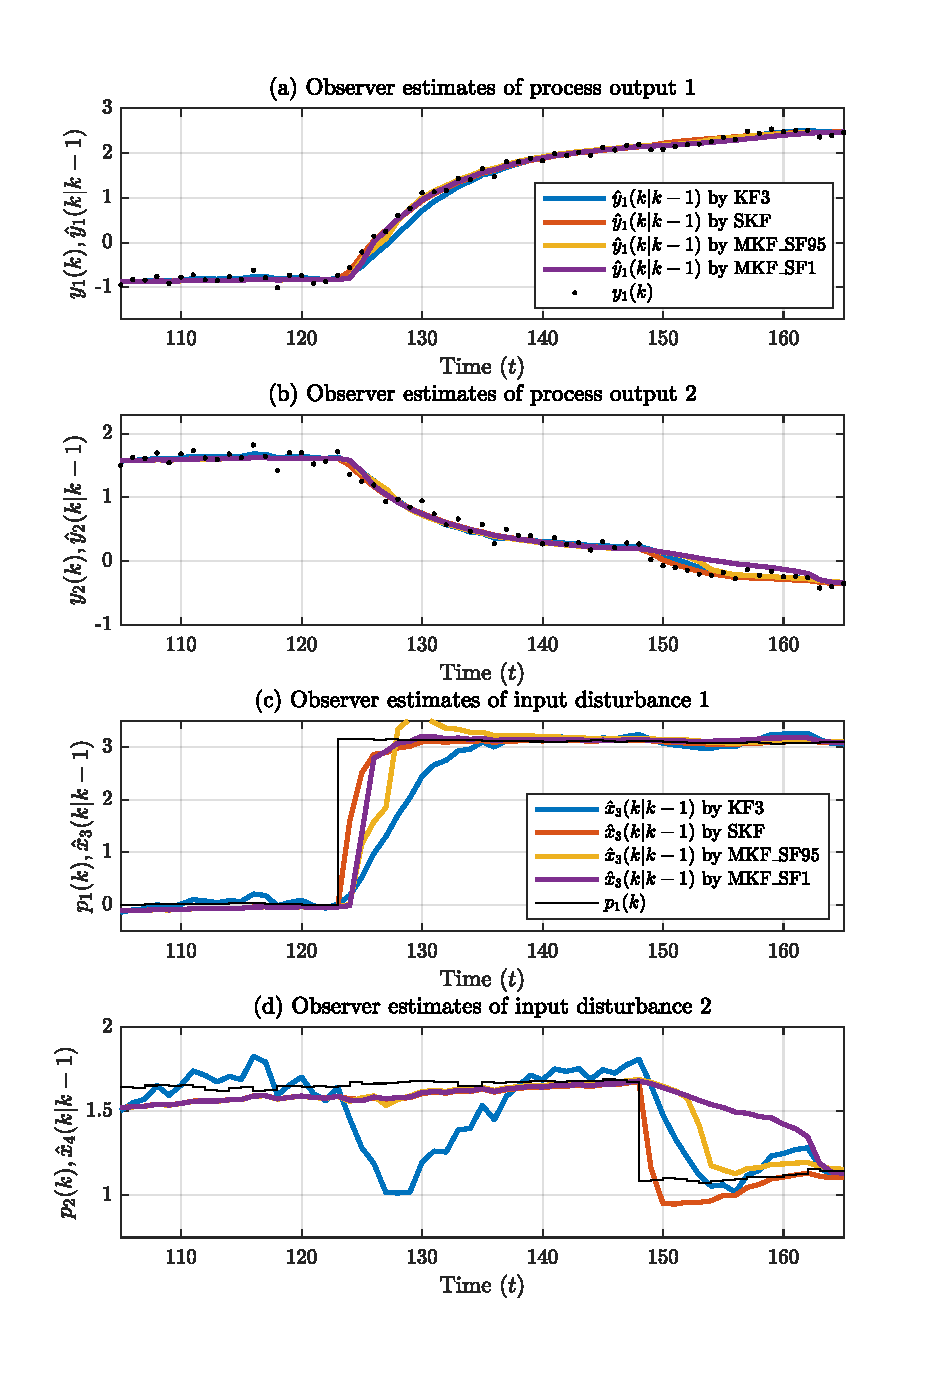
\includegraphics[width=13cm]{images/rod_obs_sim2_all_seed_y_est2_SF1.pdf}
	\caption{Estimates by sequence fusion observer –  $2\times2$ system}
	\label{fig:rod-obs-sim2-yest-2-SP}
\end{figure}

\begin{figure}[htp]
	\centering
	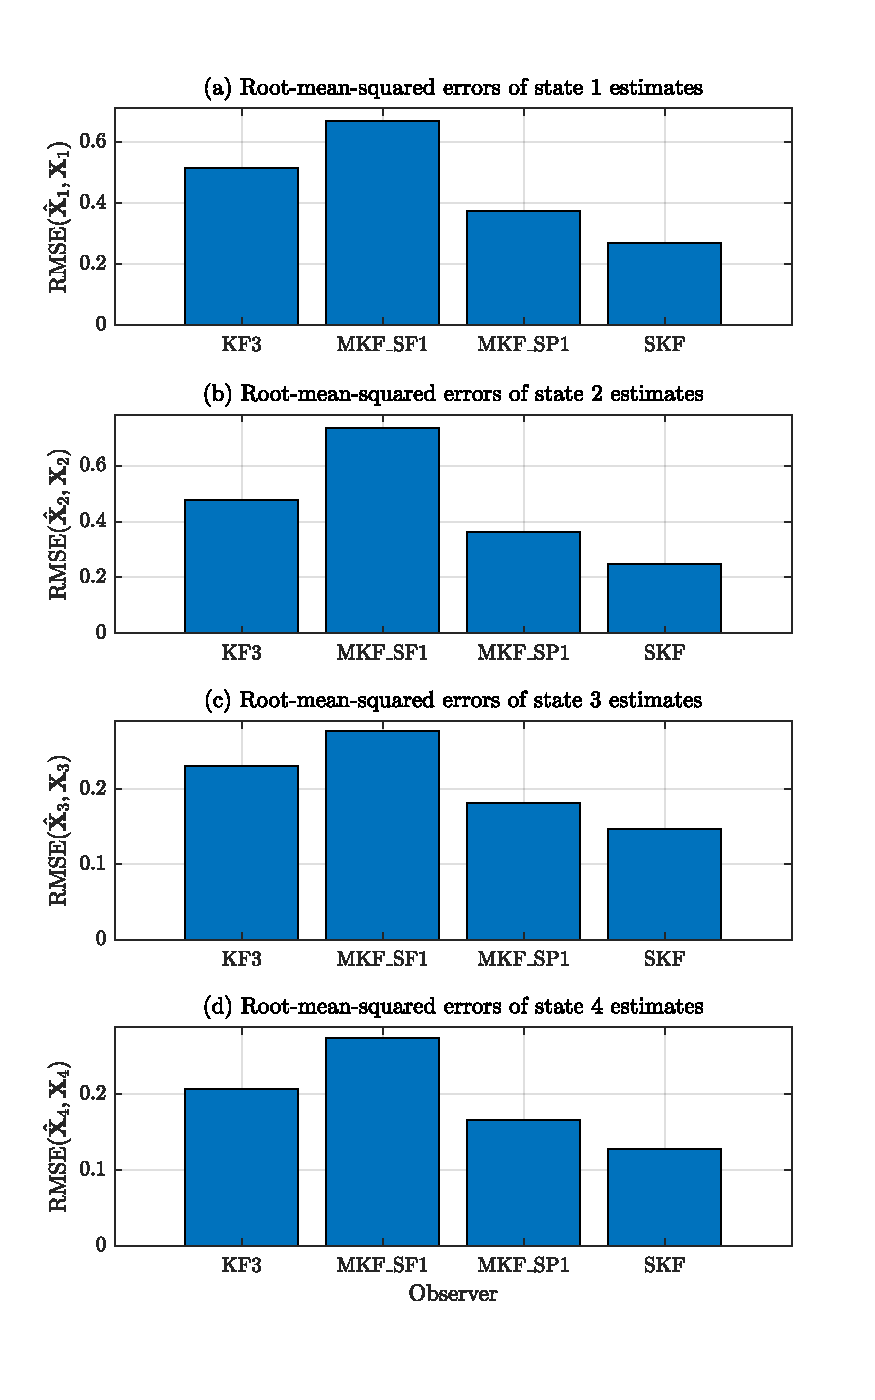
\includegraphics[width=11cm]{images/rod_obs_sim2_all_seed_x_err_bar.pdf}
	\caption{Root-mean-squared errors of state estimates – $2\times2$ system}
	\label{fig:rod-obs-sim2-xest-RMSE-bar}
\end{figure}

\begin{figure}[htp]
	\centering
	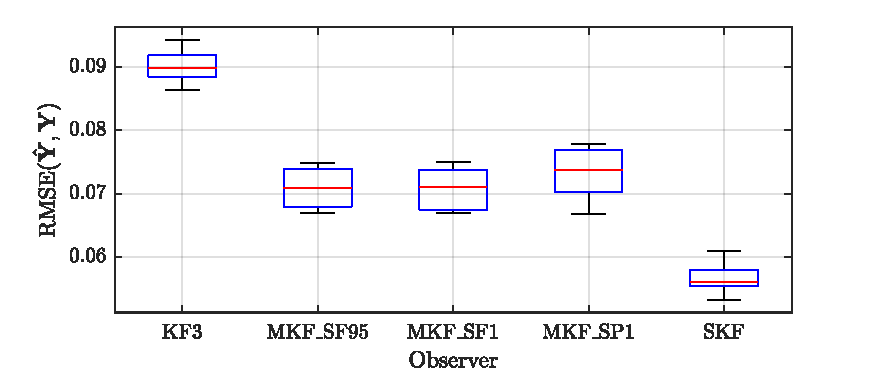
\includegraphics[width=11cm]{images/rod_obs_sim2_all_seed_y_err_box.pdf}
	\caption{Root-mean-squared errors of output estimates – $2\times2$ system}
	\label{fig:rod-obs-sim2-yest-all-seed-RMSE-box}
\end{figure}

\begin{table}[hb]
	\begin{center}
		\caption{Multi-model observer parameter search results – MKF-SF95.} \label{tb:obs-sim2-popt-SF95}
		% See: https://texblog.org/2019/06/03/control-the-width-of-table-columns-tabular-in-latex/
		\begin{tabular}{p{0.05\textwidth}>{\centering\arraybackslash}p{0.07\textwidth}>{\centering\arraybackslash}p{0.07\textwidth}>{\centering\arraybackslash}p{0.07\textwidth}>{\centering\arraybackslash}p{0.07\textwidth}>{\centering\arraybackslash}p{0.24\textwidth}}
			$n_f$ & $n_m$ & $n_d$ & $n_h$ & $\beta$ & $\operatorname{RMSE}(\hat{Y}(N),Y(N))$  \\
			\hline
			% Results with seed = 0
			30 &   2 &   2 & 466 & 0.8600 & 0.0787 \\
			30 &   2 &   3 & 211 & 0.8182 & 0.0791 \\
			30 &   3 &  10 &  42 & 0.7629 & 0.0802 \\
			30 &   2 &  10 &  22 & 0.7629 & 0.0803 \\
			50 &   3 &  10 & 176 & 0.6369 & 0.0803 \\
			45 &   2 &   3 & 466 & 0.7399 & 0.0811 \\
			25 &   3 &   5 & 176 & 0.8183 & 0.0816 \\
			25 &   2 &   5 &  56 & 0.8183 & 0.0817 \\
			20 &   2 &   2 & 211 & 0.9045 & 0.0830 \\
			15 &   2 &   1 & 466 & 0.9995 & 0.0850 \\
			\hline
		\end{tabular}
	\end{center}
\end{table}


\begin{table}[hb]
	\begin{center}
		\caption{Multi-model observer parameter search results – MKF-SF98.} \label{tb:obs-sim2-popt-SF98}
		% See: https://texblog.org/2019/06/03/control-the-width-of-table-columns-tabular-in-latex/
		\begin{tabular}{p{0.05\textwidth}>{\centering\arraybackslash}p{0.07\textwidth}>{\centering\arraybackslash}p{0.07\textwidth}>{\centering\arraybackslash}p{0.07\textwidth}>{\centering\arraybackslash}p{0.07\textwidth}>{\centering\arraybackslash}p{0.24\textwidth}}
			$n_f$ & $n_m$ & $n_d$ & $n_h$ & $\beta$ & $\operatorname{RMSE}(\hat{Y}(N),Y(N))$  \\
			\hline
			% Results with seed = 0, nT = 5000 (RMSE_y_sum)
			%45 &   2 &   3 & 466 & 0.9900 & 0.1555 \\
			%30 &   2 &   2 & 466 & 0.9967 & 0.1559 \\
			%30 &   2 &   3 & 211 & 0.9969 & 0.1559 \\
			%15 &   2 &   1 & 466 & 0.9995 & 0.1701 \\
			%50 &   3 &  10 & 176 & 0.9991 & 0.1716 \\
			%50 &   2 &  10 &  56 & 0.9892 & 0.1716 \\
			%50 &   2 &   5 & 211 & 0.9874 & 0.1737 \\
			%20 &   2 &   2 & 211 & 0.9990 & 0.1775 \\
			%5 &   1 &   1 &  11 & 0.9990 & 0.1861 \\
			%5 &   3 &   1 & 176 & 1.0000 & 0.1861 \\
			% Results with seed =0, after modification of MKF_SF98
			45 &   2 &   3 & 466 & 0.9900 & 0.0802 \\
			15 &   2 &   1 & 466 & 0.9995 & 0.0850 \\
			5 &   3 &  10 & 176 & 0.9991 & 0.0858 \\
			30 &   2 &   2 & 466 & 0.9967 & 0.0904 \\
			9 &   1 &   3 &   7 & 0.9975 & 0.0924 \\
			9 &   2 &   3 &  22 & 0.9999 & 0.0924 \\
			9 &   3 &   3 &  42 & 1.0000 & 0.0924 \\
			6 &   1 &   2 &   7 & 0.9988 & 0.0929 \\
			6 &   2 &   2 &  22 & 1.0000 & 0.0929 \\
			6 &   3 &   2 &  42 & 1.0000 & 0.0929 \\
			\hline
		\end{tabular}
	\end{center}
\end{table}

\begin{table}[hb]
	\begin{center}
		\caption{Multi-model observer parameter search results – MKF-SP.} \label{tb:obs-sim2-popt-SP}
		% See: https://texblog.org/2019/06/03/control-the-width-of-table-columns-tabular-in-latex/
		\begin{tabular}{p{0.05\textwidth}>{\centering\arraybackslash}p{0.07\textwidth}>{\centering\arraybackslash}p{0.24\textwidth}}
			$n_h$ & $n_\text{min}$ & $\operatorname{RMSE}(\hat{Y}(N),Y(N))$  \\
			\hline
			% Results with seed = 2, nT = 2500
			%19 &   5 & 0.0775  \\
			%19 &   7 & 0.0775  \\
			%25 &   6 & 0.0775  \\
			%25 &   9 & 0.0775  \\
			%32 &  12 & 0.0775  \\
			%25 &   5 & 0.0775  \\
			%25 &   7 & 0.0776  \\
			%19 &   4 & 0.0776  \\
			%32 &   9 & 0.0776  \\
			%25 &   4 & 0.0776  \\
			% Results with seed = 0, nT = 5000
			19 &   6 & 0.0408  \\
			25 &   9 & 0.0408  \\
			32 &  12 & 0.0408  \\
			19 &   4 & 0.0408  \\
			19 &   5 & 0.0408  \\
			25 &   7 & 0.0408  \\
			25 &   6 & 0.0409  \\
			32 &   9 & 0.0409  \\
			25 &   5 & 0.0409  \\
			32 &   7 & 0.0409  \\
		\end{tabular}
	\end{center}
\end{table}


\begin{table}[hb]
	\begin{center}
		\caption{Observers and parameters for $2\times2$ linear system.} \label{tb:obs-params-sim2}
		% See: https://texblog.org/2019/06/03/control-the-width-of-table-columns-tabular-in-latex/
		\begin{tabular}{p{0.16\textwidth}>{\centering\arraybackslash}p{0.11\textwidth}>{\centering\arraybackslash}p{0.11\textwidth}>{\centering\arraybackslash}p{0.11\textwidth}>{\centering\arraybackslash}p{0.16\textwidth}>{\centering\arraybackslash}p{0.16\textwidth}}
			& KF1 & KF2 & KF3 & MKF-SF1 & MKF-SP1 \\
			\hline
			Type & Kalman filter & Kalman filter & Kalman filter & Multi-model Kalman filter & Multi-model Kalman filter \\
			Sub-optimal algorithm & - & - & - & Sequence fusion & Sequence pruning \\
			\hline
			Parameters &  &  &  & &  \\
			$\mathbf{Q}$ & $\mathbf{Q}_0$ & $\mathbf{Q}_1$ & $\mathbf{Q}_{opt}$ & $\{\mathbf{Q}_0,\mathbf{Q}_1\}$ & $\{\mathbf{Q}_0,\mathbf{Q}_1\}$ \\
			$\mathbf{R}$ & $\left[\begin{smallmatrix}0.1^2 & 0 \\ 0 & 0.1^2\end{smallmatrix}\right]$
				& $\left[\begin{smallmatrix}0.1^2 & 0 \\ 0 & 0.1^2\end{smallmatrix}\right]$
				& $\left[\begin{smallmatrix}0.1^2 & 0 \\ 0 & 0.1^2\end{smallmatrix}\right]$
				& $\left[\begin{smallmatrix}0.1^2 & 0 \\ 0 & 0.1^2\end{smallmatrix}\right]$
				& $\left[\begin{smallmatrix}0.1^2 & 0 \\ 0 & 0.1^2\end{smallmatrix}\right]$ \\
			$\mathbf{P}(0)$ & $\mathbf{P}_0$ & $\mathbf{P}_0$ & $\mathbf{P}_0$ & $\mathbf{P}_0$ & $\mathbf{P}_0$ \\
			No. of filters & 1 & 1 & 1 & 56 & 19 \\
			$n_f$ & - & - & - & 25 & - \\
			$n_m$ & - & - & - & 2 & - \\
			$n_d$ & - & - & - & 5 & - \\
			$n_{min}$ & - & - & - & - & 5 \\
			$\epsilon$ & - & - & - & 0.005 & 0.005 \\
			$\sigma_{w_p}$ & - & - & - & 0.01 & 0.01 \\
			$b$ & - & - & - & 100 & 100 \\
			\hline
		\end{tabular}
	\end{center}
\end{table}

\begin{figure}[htp]
	\centering
	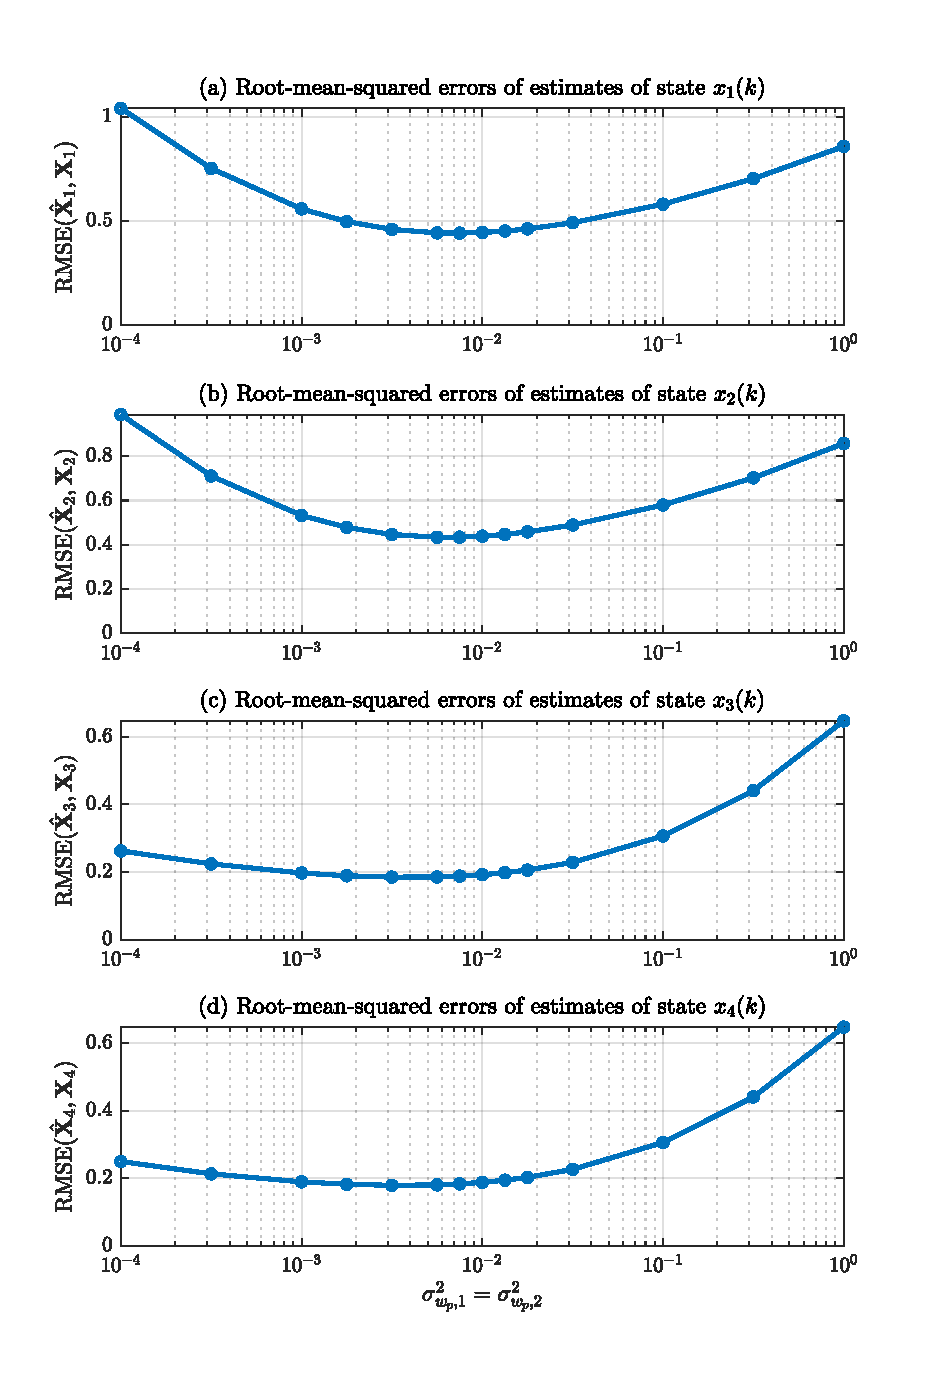
\includegraphics[width=13cm]{images/rod_obs_sim2_3KF_Q_seed_0.pdf}
	\caption{Tuning of Kalman filter KF3 – $2\times2$ linear system}
	\label{fig:sim-sys-siso--KF3-tuning}
\end{figure}

\begin{itemize}
	\item Summary table comparing performance metrics for all three observers (KF3, MKF-SF, MKF-SP) - metrics: MSE, MSE-transitions, MSE-steady-state, variance-steady-state, MSD-steady-state.
	\item Discussion: Compare and contrast -> sequence pruning approach (Eriksson and Isaksson) works better.
	\item Conclude on pros, cons of each algorithm and decision to use sequence pruning for grinding simulation experiments.
\end{itemize}

\section{Ore feed disturbance estimation} \label{section:sim-ore-SISO}

Outline notes:
\begin{outline}
	\1 Unlike previous simulations, this is a non-linear model.
	\1 Describe simulations with grinding simulation model with changing ore properties and changes (same as IFAC paper).
	\1 Describe various data sets generated and their intended use (estimation, validation, statistical performance evaluation).
	\1 Data set used for model identification in Figure: Input-output data – Figure \ref{fig:rod_obs_sim_1_ioplot_P2DcTd4}.
	\1 How process model was identified.
	\1 Augmented model with RODD input step disturbance.
	\1 Use best observer from previous section (sequence pruning).
	\1 Table showing observer paramters.
	\1 Figure: comparison of observer estimates – Figure \ref{fig:rod_obs_sim_1_est_P2DcTd4}.
	\1 Figure: Observer responses to disturbances – Figure \ref{fig:sim_resp_plot}.
	\1 Describe overall performance comparison using metrics in Table \ref{tb:results}.
	\1 Discuss pro's and con's of MKF observer (steady-state errors vs error in transitions, etc.)
	\1 Discuss applications and potential benefits (e.g. process control, RTO).
	\1 Describe sensitivity analysis simulations.
	\1 Describe sensitivity results:
	\2 (1) to model error, compare Kalman filter and MKF. Figures \ref{fig:rod_obs_sim_sens_model_KF2_MSE_y_est} and \ref{fig:rod_obs_sim_sens_model_MKF_MSE_y_est}.
	\2 (2) MKF sensitivity to RODD model parameters. Figure  \ref{fig:rod_obs_sim_sens_rod_MKF_MSE_y_est}
\end{outline}

\begin{figure}[htp]
	\centering
	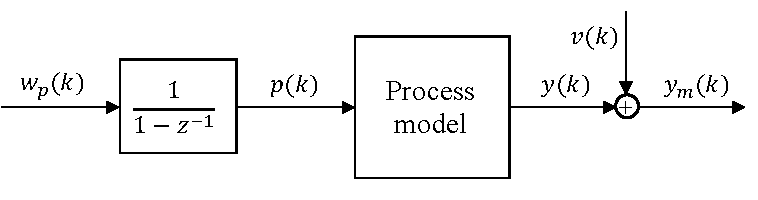
\includegraphics[width=10cm]{images/obs-model-diag.pdf}
	\caption{Observer model structure}
	\label{fig:obs_model}
\end{figure}

\begin{figure}[htp]
	\centering
	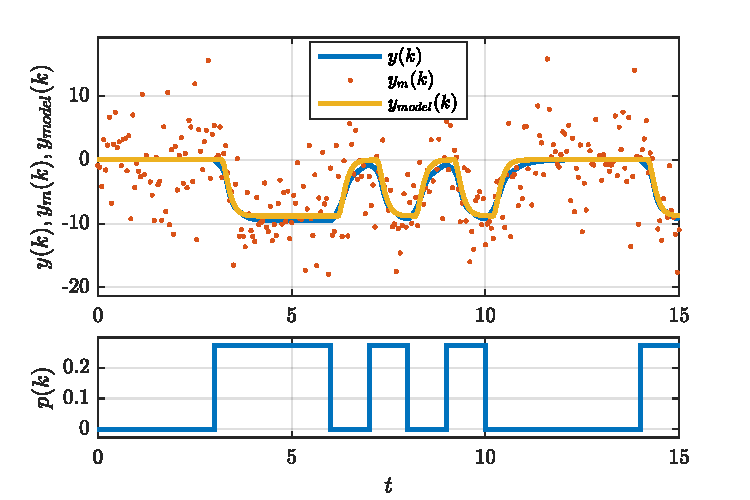
\includegraphics[width=12cm]{images/rod_obs_sim_1_ioplot_P2DcTd4.pdf}
	\caption{Grinding process simulation data and model estimates}
	\label{fig:rod_obs_sim_1_ioplot_P2DcTd4}
\end{figure}

\begin{figure}[htp]
	\centering
	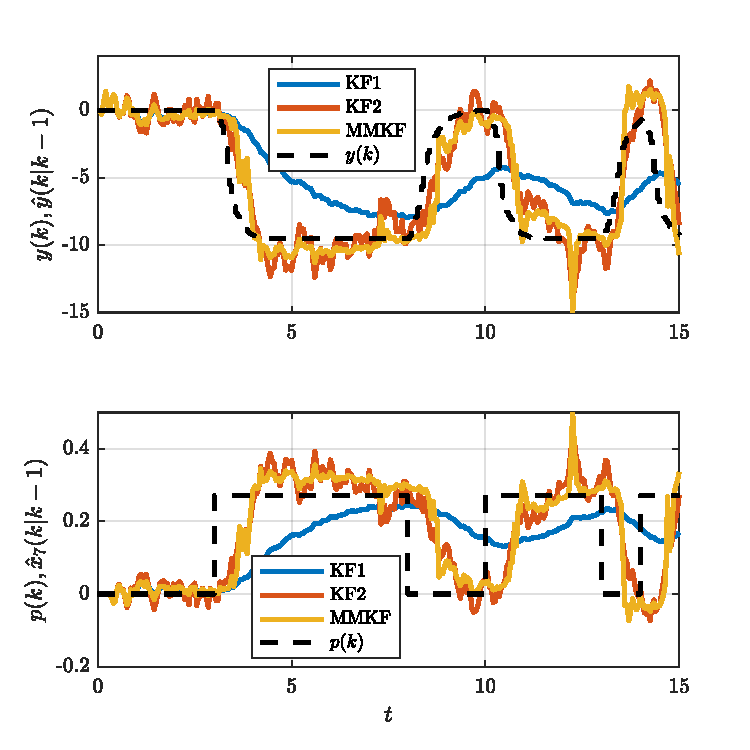
\includegraphics[width=12cm]{images/rod_obs_sim_1_est_P2DcTd4.pdf}
	\caption{Observer estimates}
	\label{fig:rod_obs_sim_1_est_P2DcTd4}
\end{figure}

\begin{figure}[htp]
	\centering
	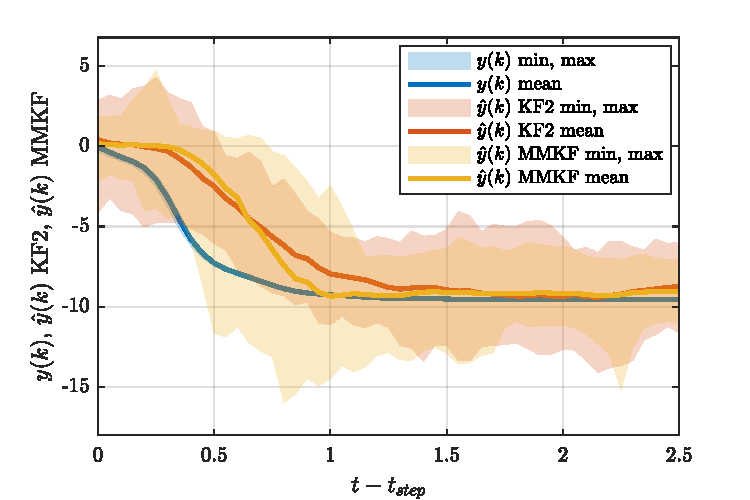
\includegraphics[width=12cm]{images/sim_resp_plot1_P2DcTd4.pdf}
	\caption{Average observer responses to step disturbances}
	\label{fig:sim_resp_plot}
\end{figure}

\begin{table}[hb]
	\begin{center}
		\caption{Observer performance evaluation metrics.} \label{tb:results}
		% See: https://texblog.org/2019/06/03/control-the-width-of-table-columns-tabular-in-latex/
		\begin{tabular}{p{0.34\textwidth}>{\centering\arraybackslash}p{0.09\textwidth}>{\centering\arraybackslash}p{0.09\textwidth}>{\centering\arraybackslash}p{0.09\textwidth}>{\centering\arraybackslash}p{0.11\textwidth}>{\centering\arraybackslash}p{0.09\textwidth}}
			Metric & KF1 & KF2 & KF3 & MKF-SP & SKF \\
			\hline
			MSE($\hat{y}(k),y(k)$) overall          & 11.0 & 15.9 & 3.7 & 3.5 & 2.1 \\ 
			MSE($\hat{y}(k),y(k)$) transient       & 21.1 & 16.1 & 7.7 & 11.2 & 5.1 \\ 
			MSE($\hat{y}(k),y(k)$) steady-state & 7.9 & 15.9 & 2.5 & 1.1 & 1.1 \\ 
			Var($\hat{y}(k)$) steady-state          & 1.8 & 15.3 & 1.9 & 0.5 & 0.2 \\ 
			MSD($\hat{y}(k),y(k)$) steady-state       & 0.0 & 16.2 & 0.5 & 0.2 & 0.0 \\ 
			% Results for P2DcTd4
			%  Gc = -32.4 * exp(-0.2 * s) / (1 + 0.106*s)^2;
			%                                 KF1       KF3       AFMM        SKF  
			%  MSE                         11.118    3.7395     3.6991     2.0615
			%  MSE in transitions          20.687    7.7201      12.18     5.0674
			%  MSE in steady-state         8.1885     2.521     1.1028     1.1414
			%  Variance in steady-state    1.7723    1.9026    0.39281    0.23769
			%
			% Results for P2Dcd1_T
			%  Gc = -35.94 * exp(-0.05 * s) / ((1 + 0.235*s) * (1 + 0.161*s));
			%                                 KF1       KF3       AFMM        SKF  
			%  MSE                         10.707    3.7702     3.7283     1.9652
			%  MSE in transitions          21.052    7.7605     12.397     4.8145
			%  MSE in steady-state         7.5404    2.5486     1.0745      1.093
			%  Variance in steady-state    1.8111    1.9259    0.39282    0.24514
			
			% Updated results for P2DcTd4 with n_filt = 20, n_min = 18 after fixing
			% initialization between MC simulation runs.
			%  MSE                          11.01    3.6869     3.4952     1.8191
			%  MSE in transitions          21.137    7.7201     11.208     5.0722
			%  MSE in steady-state         7.9091    2.4523     1.1342     0.8232
			%  Variance in steady-state    1.8008    1.9026    0.47604    0.23759
			
			\hline
		\end{tabular}
	\end{center}
\end{table}

\begin{figure}[htp]
	\centering
	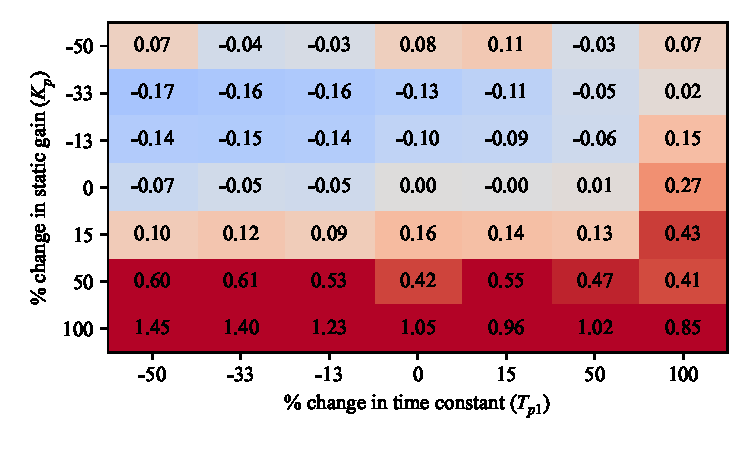
\includegraphics[width=12cm]{images/rod_obs_sim_sens_model_KF2_MSE_y_est.pdf}
	\caption{Sensitivity of KF2 estimates to changes in model parameters}
	\label{fig:rod_obs_sim_sens_model_KF2_MSE_y_est}
\end{figure}

\begin{figure}[htp]
	\centering
	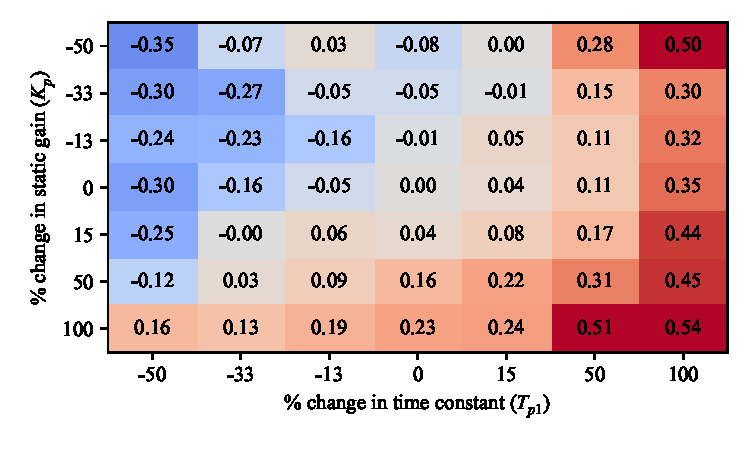
\includegraphics[width=12cm]{images/rod_obs_sim_sens_model_MKF_MSE_y_est.pdf}
	\caption{Sensitivity of MKF observer estimates to changes in model parameters}
	\label{fig:rod_obs_sim_sens_model_MKF_MSE_y_est}
\end{figure}

\begin{figure}[htp]
	\centering
	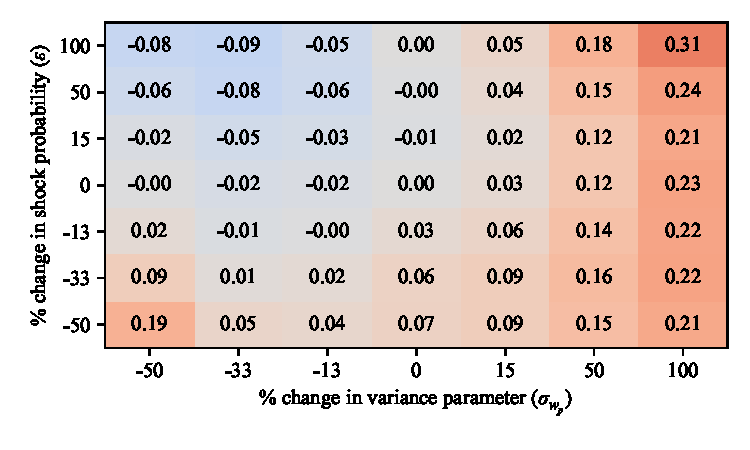
\includegraphics[width=12cm]{images/rod_obs_sim_sens_rod_MKF_MSE_y_est.pdf}
	\caption{Sensitivity of MKF observer estimates to changes in RODD parameters}
	\label{fig:rod_obs_sim_sens_rod_MKF_MSE_y_est}
\end{figure}


\section{Grinding circuit control simulation} \label{section:sim-ore-mimo-ctrl} 

Outline notes:
\begin{itemize}
	\item Grinding simulation model in closed loop with MPC controller.
	\item Diagram of feedback system – Figure \ref{fig:sim-mpc-diag}
	\item Table of results - Performance metrics — e.g. tracking error.
	\item Robustness?  E.g. stability margins.
\end{itemize}

\begin{figure}[htp]
	\centering
	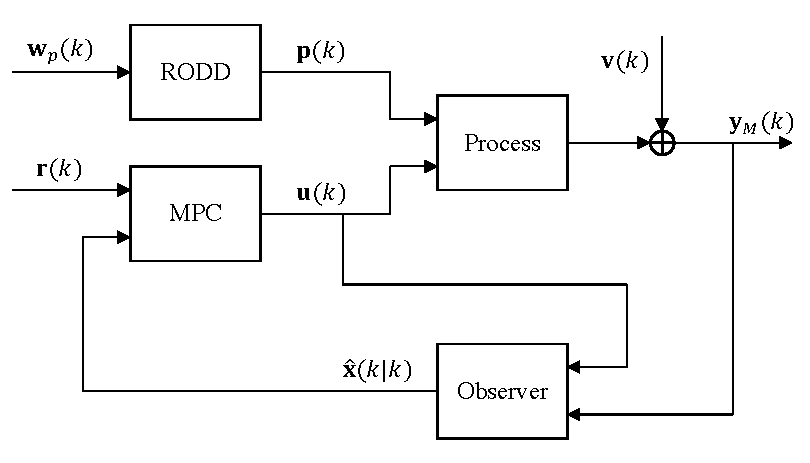
\includegraphics[width=12cm]{images/sim-mpc-diag.pdf}
	\caption{Functional diagram of the simulated feedback control system}
	\label{fig:sim-mpc-diag}
\end{figure}